\chapter{Theory: How to calculate grating efficiency}
\section{Introduction to grating theory}
\begin{figure}[htbp] %  figure placement: here, top, bottom, or page
   \centering
   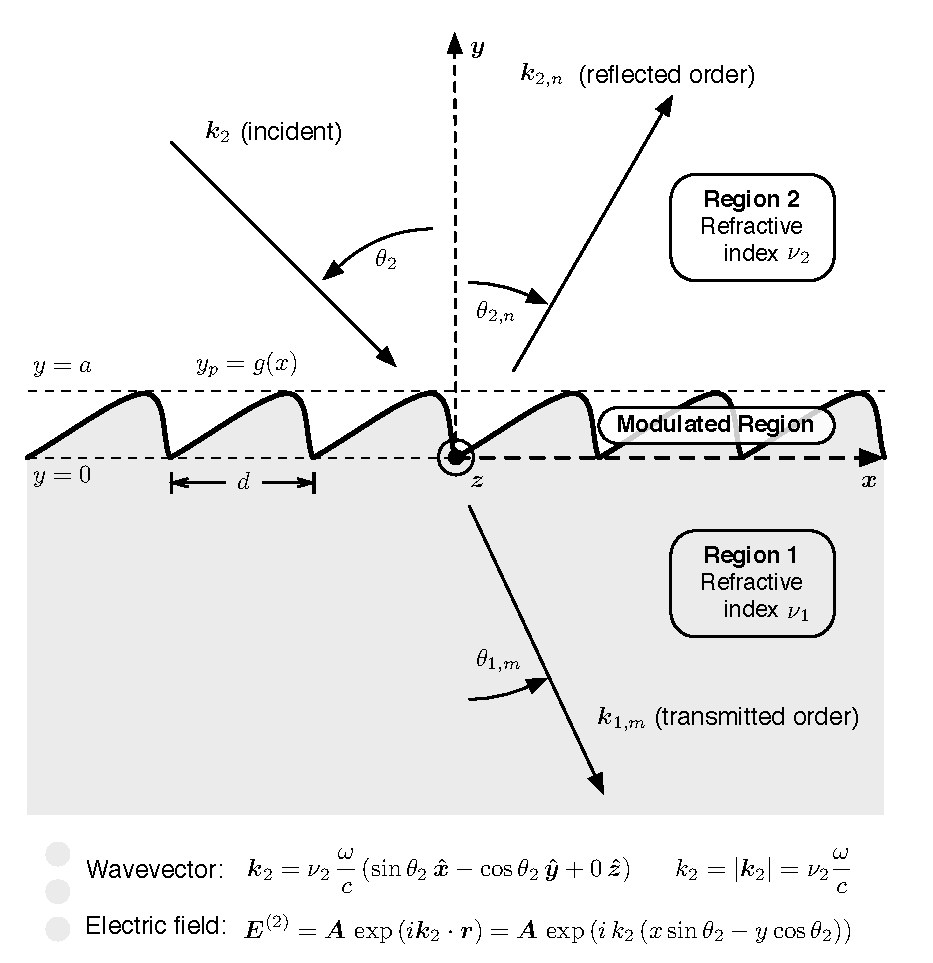
\includegraphics[scale=0.8]{Chapter2/2a_inPlaneIncidence/2a.pdf} 
   \caption{A one-dimensional grating with in-plane incidence.}
   \label{2a}
\end{figure}
For centuries, we have known that gratings reflect and transmit light at a set of discrete angles -- called \emph{orders} -- where the angles depend on the wavelength  (Figure \ref{2a}).  A variety of simple proofs have been used to explain this.  In undergraduate books, the grating equation is introduced as a consequence of constructive interference from a linear array of coherent emitters. (This makes sense for a slotted transmission grating, but it is less obvious why an arbitrarily-shaped periodic reflecting structure 
%TODO like one of those shown in Figure \ref{3c-profile} would behave the same way.)  
like the one in Figure \ref{3a} would behave the same way.)  
Other proofs -- such as those using Fermat's Principle to minimize an optical path function with a phase offset introduced by the grating \cite[p.~93 -- 99]{Pea97} -- are general enough to explain the existence of diffraction orders, but they do not say anything about how much light goes into each.

This is unfortunate, because to determine grating efficiency, we must determine the intensity of the orders.  A huge amount of research has gone into this question since Lord Rayleigh's pioneering work in 1907 \cite{Ray07}, and some clever analytical methods were even discovered that simplify the problem -- but only for certain special groove shapes.  It is only within the last twenty years that mathematical techniques and computational power have advanced enough to accurately model the electromagnetic field of light within and near the surface of an arbitrary grating, allowing us to actually determine how energy is distributed between the orders, and how much is absorbed within the grating.  In this chapter, we look at a history of the key developments in grating theory, give a comparison of the current methods, and then set up the grating problem using the most general of these methods.

\subsection{A brief history of grating theory}

We define the ``grating problem'' as the problem of determining the intensity of a grating's reflected and transmitted light everywhere.  In general, this requires finding the solution to Maxwell's equations for the electric and magnetic fields of the light, in the presence of the grating's periodic boundary conditions, for a known incident field.  

Prior to the availability of computers and numerical techniques, great attempts were made to solve this problem analytically.  In 1907, Lord Rayleigh set up the problem\footnote{Actually, Rayleigh's first application of this technique was to the diffraction of sound waves \cite{Ray86}.  It turns out that the wave equation for a pressure wave in compressible media is the same as for the fields in an electromagnetic wave, and the boundary conditions at interfaces are also analogous. In Reference \cite{Ray07} he shows applications to both sound and light.} using a Fourier approach identical to the one we use later in this chapter \cite{Ray07}.  However, without access to powerful numerical methods, he could only make coarse approximations, using expansions truncated at the first or second power of the groove height.\footnote{And this, despite assuming a perfectly reflecting grating, exactly normal incidence, and only one term in the Fourier expansion for the groove shape -- i.e., a sinusoidal grating.}  This led to some obviously non-physical results, such as predictions of infinite intensity in any order when the outgoing angle of a higher order reached exactly 90 degrees.  From 1907 until 1960, advancements in grating theory amounted to finding clever but limited simplifications to these expansions, which would work in the case of one particular groove profile, incidence angle, or approximation limit.

The introduction of computer-based numerical methods in the 1960s spawned a renewal of research into general solutions to the problem.  The first ``rigorous'' algorithm\footnote{``Rigorous'' here implies a method that does not introduce approximations into the theoretical equations, other than inevitably in the process of finite-precision numerical calculations.} was invented by several researchers in 1966:
\begin{description}
\item[The ``integral'' approach] uses Maxwell's equations in integral form and the Kirchhoff integral theorem \cite{Pet66}\cite{Wir69}\cite{Pav70}.  It was generalized from perfectly conducting (i.e.: perfectly reflecting) gratings to finite-conductivity metallic gratings in an important paper in 1972 \cite{May72}.
\end{description}
Alongside these ``integral'' methods, two other broad families of algorithms emerged based on Maxwell's equations in differential form:
\begin{description}
\item[The ``modal'' method] relates the electromagnetic field to a Fourier expansion in the vertical ($y$) direction with unknown coefficients, called modes. The total field satisfying the boundary conditions is solved algebraically as a linear combination of the modes \cite{Bot81}\cite{Bot81a}\cite{And81}.
\item[The ``differential'' methods] exploit the periodicity of the grooves to express both the grating boundary and the fields as Fourier expansions in the $x$-direction. The total field satisfying the boundary conditions is determined by numerically integrating a finite set of differential equations. (We explore the details of this method later in this chapter.)
\end{description}
The modal methods are not actually general because in their application of the boundary conditions, they require the edges of the grooves to be vertical; this limits them to rectangular gratings.  However, they are accurate in this special case, and fast compared to the differential method because they avoid numerical integration.  
The other two approaches are general in representation, although the stability and accuracy of the integral approach is highly contingent on the groove geometry.

By 1980, grating theorists had devised a wide variety of implementations for each family.  % -- after all, it is one matter to express the problem as a complete set of algebraic or differential equations; it is another matter to actually solve that set!
Reference \cite{Pet80} provides a comprehensive review of all the methods that were available by this date.\footnote{The same author provides a follow-up paper, written ten years later on new methods that differ completely from the fundamentals used in 1980 \cite{Pet90}.}  Of the three families, the differential approach had proven to be the most general way of setting up the problem, but it ran into two numerical issues -- particularly when used to describe TM-polarized light on highly-conducting metallic gratings.  One issue was strictly computational: round-off errors when doing finite-precision computer arithmetic would lead to growing contamination during the numerical integration of exponential functions.  This problem was solved by the introduction of the ``S-matrix'' propagation algorithm in 1996 \cite{Li96}\cite{Mon98}.  The second problem was related to the mathematical implications of truncating an infinite Fourier series -- unfortunately but obviously necessary for numerical calculations.  This challenge was also finally resolved by the breakthrough work of Li \cite{Li96b} in 1996 on the factorization of truncated Fourier series, and has been applied extensively by Neviere and Popov both to the simple cases of one-dimensional gratings like those shown in Figure \ref{2a} \cite{Pop01}, and to complex three-dimensional periodic structures of anisotropic materials \cite{Pop00}\cite{Nev02}.

\subsection{Comparison and applicability of grating theory families}
\label{methodComparison}
To choose an appropriate method for a particular problem, we need to understand the assumptions and limitations of each one.  As a ``grating method user's guide'', this section presents just enough theory to understand their areas of applicability.  We cover the integral method, the modal method, and two variations of the differential method.  This survey is not exhaustive; additional methods have been developed that are only applicable in specific cases.  For example, for certain particular groove profiles, there exist coordinate transformations and ``conformal mappings'', which simplify the boundary conditions so that the grating problem can either be solved analytically, or reduced in complexity.  We concentrate here on the methods that have been intended for general applications.
\subsubsection{The Integral Method}
For perfectly conducting metals, when an electromagnetic field is incident on a surface, it induces a surface current $\mathbf{j}_S(\mathbf{M}')$ at each point $\mathbf{M}'$.  This surface current radiates a field -- the diffracted electric field $E(P)$ at a given point $\mathbf{P}$ above the surface; the field is related to the surface current by the Kirchhoff Integral Theorem \cite{Kir83} using the Green's function $G(\mathbf{P}, \mathbf{M}')$:
\begin{align}
\mathbf{E}(\mathbf{P}) = \int\limits_{\textrm{grating period}} G(\mathbf{P}, \mathbf{M}')\, \phi(\mathbf{M}')\, \dif s'
\end{align}
where $\dif s$ is a curvilinear coordinate along the grating profile, and $\phi(\mathbf{M'})$ is proportional to the surface current.  Unfortunately, this becomes tricky, because the surface current is not only induced by the incident electric field, but also by the diffracted field radiated from all other points along the grating surface.  This means that the surface current $\mathbf{j}_S(\mathbf{M}')$ at $\mathbf{M}'$ depends not on the incident field, but also on the current $\mathbf{j}_S(\mathbf{M}'')$ at all coordinates $\mathbf{M}''$.  By substituting the corresponding $\phi(\mathbf{M'})$ into the equation above, this transforms it into not a differential equation, but an integral equation for $\phi(\mathbf{M'})$.  
 
\noindent\textbf{\emph{Limitations}}\\
In practice, the numerical techniques required to solve this integral equation can be complicated, depending on the shape of the profile.  For imperfectly-conducting gratings, the problem becomes even more difficult, and even harder still when the grating is made up of one or many layers -- such as over-coated soft x-ray gratings and multilayers.  Although it is universal, the main limitation of the integral approach is its computational cost, and the programming difficulty of applying it correctly to every unique grating situation. Numerical challenges abound, particularly regarding the discretization of the grating profile and how sharp corners and discontinuities are handled.  Reference \cite{Pom91} presents an overview of integral implementations, as well as approximations for reducing the computation time and handling coating layers. The latest version -- referred to as the ``modified integral method'' by Goray, has been the topic of many recent publications \cite{Gor02} \cite {Gor02b} \cite{See02} \cite{Gor05}.
 
\subsubsection{Methods using Maxwell's Equations in differential form}
The remaining two families (the modal method and the differential method) start from Maxwell's equations in differential form.  Within the differential method, there are two variants: the ``classical'' differential method, and the ``Rigorous Coupled Wave'' (RCW) approach.  We present all three here together because they share the same foundation.  They all start by projecting the solution to Maxwell's Equations -- i.e., the strength of the electric or magnetic field of the waves -- onto some periodic basis in the $x$-direction, but with an unknown dependence on $y$.  The task for each method is to determine the $y$-dependence by ensuring the total field satisfies the boundary conditions on the grating surface and at infinite.  The modal method and the RCW method both assume a rectangular groove profile, so that the boundary conditions are simplified: this implies that the tangential and normal field components at the grating interface are purely along either the $x$ or $y$-direction.
\begin{description}
\item[The modal method] assumes a basis of functions that are periodic in $x$, with ``modes'' $F_m$ related to the field $u_m(x)$ as
\begin{align}
F_m(x,y)=u_m(x) \, \exp \left( i \rho_m y \right)
\end{align}
where $\rho_m$ is a ``mode constant''.  The total field is assumed to be a linear combination of the modes with unknown amplitudes, and since this field must satisfy the boundary conditions on the surface, it is possible to create a set of linear algebraic equations that can be solved for the mode amplitudes.
 
\noindent\textbf{\emph{Limitations}}\\
For the modal method, the number of modes and the mode constants $\rho_m$ must be sufficient to fully describe the actual field.  For highly conducting materials, finding appropriate mode constants is difficult, but a technique is available in Reference \cite{And81}.  
 
The other obvious limitation of the modal method is to rectangular gratings with vertical groove boundaries.  We can attempt to avoid this limitation by using stacks of thin rectangular gratings to represent an arbitrary shape, as shown in Figure \ref{3a}.  This is called the ``staircase approximation'' for obvious reasons, and is also used in the RCW method.  Unfortunately, no matter how thin the slices are made, this approximation creates sharp edges between the layers at the stair-step corners.  Popov et. al. discovered that for TM-polarized light, this creates unrealistically strong electric fields at the corners, which cannot be physically representative of the true electric field near a smooth grating.  Therefore, algorithms that use the staircase approximation require a larger number of basis components to represent this abruptly changing field, which slows down the computation.  More importantly, even when there are enough components to let the solution converge, the results are not representative of reality. \cite{Pop02} 
 
\begin{figure}[tbp] %  figure placement: here, top, bottom, or page
   \centering
   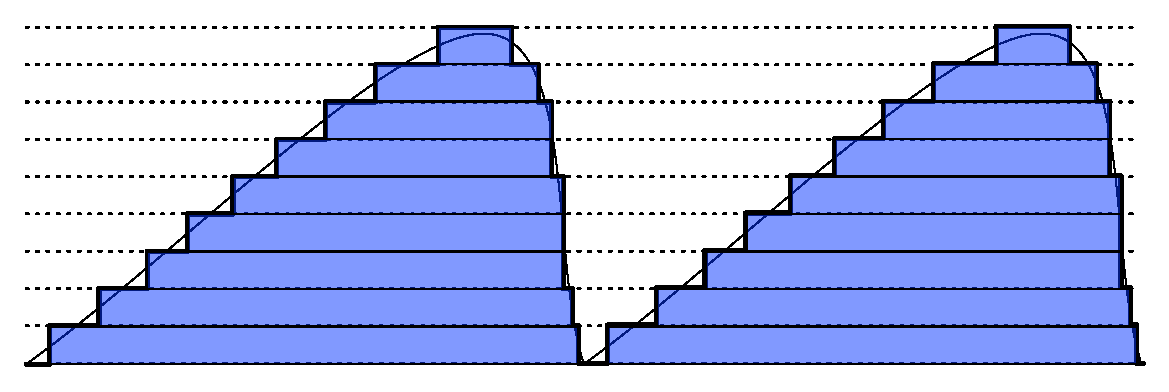
\includegraphics[scale=0.5]{Chapter3/3a_RCWA/3a.pdf} 
   \caption[The modal method and the RCW method approximate every real grating as a stack of rectangular gratings.]{The modal method and the RCW method approximate every real grating as a stack of rectangular gratings.  This simplifies the boundary conditions (the normal and tangential field components line up either along the $x$- or $y$-axis), so that the problem can be reduced to an algebraic solution for the eigenvalues of the modes or the Fourier coefficients.  Every layer is treated as a separate grating with its own effect on the incoming and outgoing fields; the total grating effect is propagated up the stack using matrix methods.}
   \label{3a}
\end{figure}
 
\item[The differential method's ``classical solution''] uses a periodic field similar to the modal method, except that the basis functions are Fourier expansions in the $x$-direction, and the unknown functions to solve are along the $y$-direction:
\begin{align}
F(x,y)=\exp\left( ik\, \sin \theta_{2}x \right) \sum\limits_m F_m(y) \exp \left( \frac{2\pi i x}{d} \right)
\end{align}
By matching the total field to the boundary conditions at the top and bottom of the grooves, a set of coupled differential equations is created; this set is solved using a combination of numerical integration and linear algebra, which we describe later in this chapter.  
 
\noindent\textbf{\emph{Limitations}}\\
The advantage of the classical differential method is that it works for arbitrary groove profiles.  However, for rectangular profiles, it is slower than the other two options because of the necessity to perform a numerical integration for each basis component.  The pure differential method originally suffered from numerical convergence problems in TM polarization on conductive gratings, but these were resolved in 1996 \cite{Li96b} \cite{Pop00}.  The only remaining limitation is that the method assumes the material can be described by a well-behaved complex dielectric constant (or the related refractive index) both above and inside the grating material.  This rules out ``perfectly conducting'' (i.e., perfectly reflecting) gratings, for which it is not reasonable to assign a dielectric constant.  This limitation results in a numerical instability when trying to work with nearly perfectly conducting gratings -- for example, gold and aluminum metallic gratings used with deep infrared or millimetre light -- where the real part of the refractive index falls below 0.1.  (A few suggestions have been proposed recently for extending the differential method to highly conducting gratings, such as by substituting a finite-thickness perfectly-conducting layer above an absorbing substrate. \cite{Pop04})
 
Because this method conducts a numerical integration using assumed starting values along the $y$-direction from the bottom to the top of the grooves, if the grooves are very deep, the long integration distance increases the computation time.  The stability of the numerical integration process also suffers, because the exponential functions grow to span the precision available with standard floating-point ('double') variables.   Therefore, the speed and accuracy of the basic differential method are only acceptable for gratings with a low depth-to-period ratio.\footnote{This limitation is not strictly limited to the differential approach; it affects the numerical integration of the integral method as well.}  Fortunately, the stability issue can be solved using the S-matrix modification to the differential method (Section \ref{SMatrixMethod}).
 
\item[The differential method's ``Rigorous Coupled Wave'' approach] is a simplification that can be applied for rectangular gratings.  As we mentioned in the case of the modal method, when the groove edges are vertical, the boundary conditions within the grooves are invariant along the $y$-direction.  This means that an eigenvalue technique can be used instead of a full numerical integration along $y$, which reduces the problem to an algebraic solution, speeds up the calculation, and removes the numerical challenges associated with integrating growing exponentials.  As soon as this simplification was proposed, various authors \cite{Bur66} \cite{Pen75} \cite{Moh81} assumed that it could be generalized to arbitrary groove profiles by approximating them with rectangular slices, which could be made as thin as required for a given accuracy; this is the same ``staircase approximation'' used in the modal method (Figure \ref{3a}).  The RCW approach was used extensively for thirty years, and has been shown to produce fast and accurate results for TE-polarized light on dielectric and absorbing gratings.  However, as we mentioned above, the fundamental validity of the staircase approximation was challenged in Reference \cite{Pop02}.
 
\noindent\textbf{\emph{Limitations}}\\
As a differential method, the RCW approach is limited to finitely-conducting materials.  It is also limited to rectangular gratings, or (using the staircase approximation) to stacks of rectangular layers in TE polarization.  It can also produce approximate results in TM polarization for dielectric gratings.
\end{description}
 
Figure \ref{2e} gives a visual comparison of the limitations and strengths of all four techniques.  It shows that in general there is no clear ``home-run'' universal method; the techniques are complementary rather than supplementary.  The optimal choice for a particular class of grating problems depends on the overlap between the grating characteristics and the limitations of each method.
 
\begin{figure}[htbp] %  figure placement: here, top, bottom, or page
   \centering
   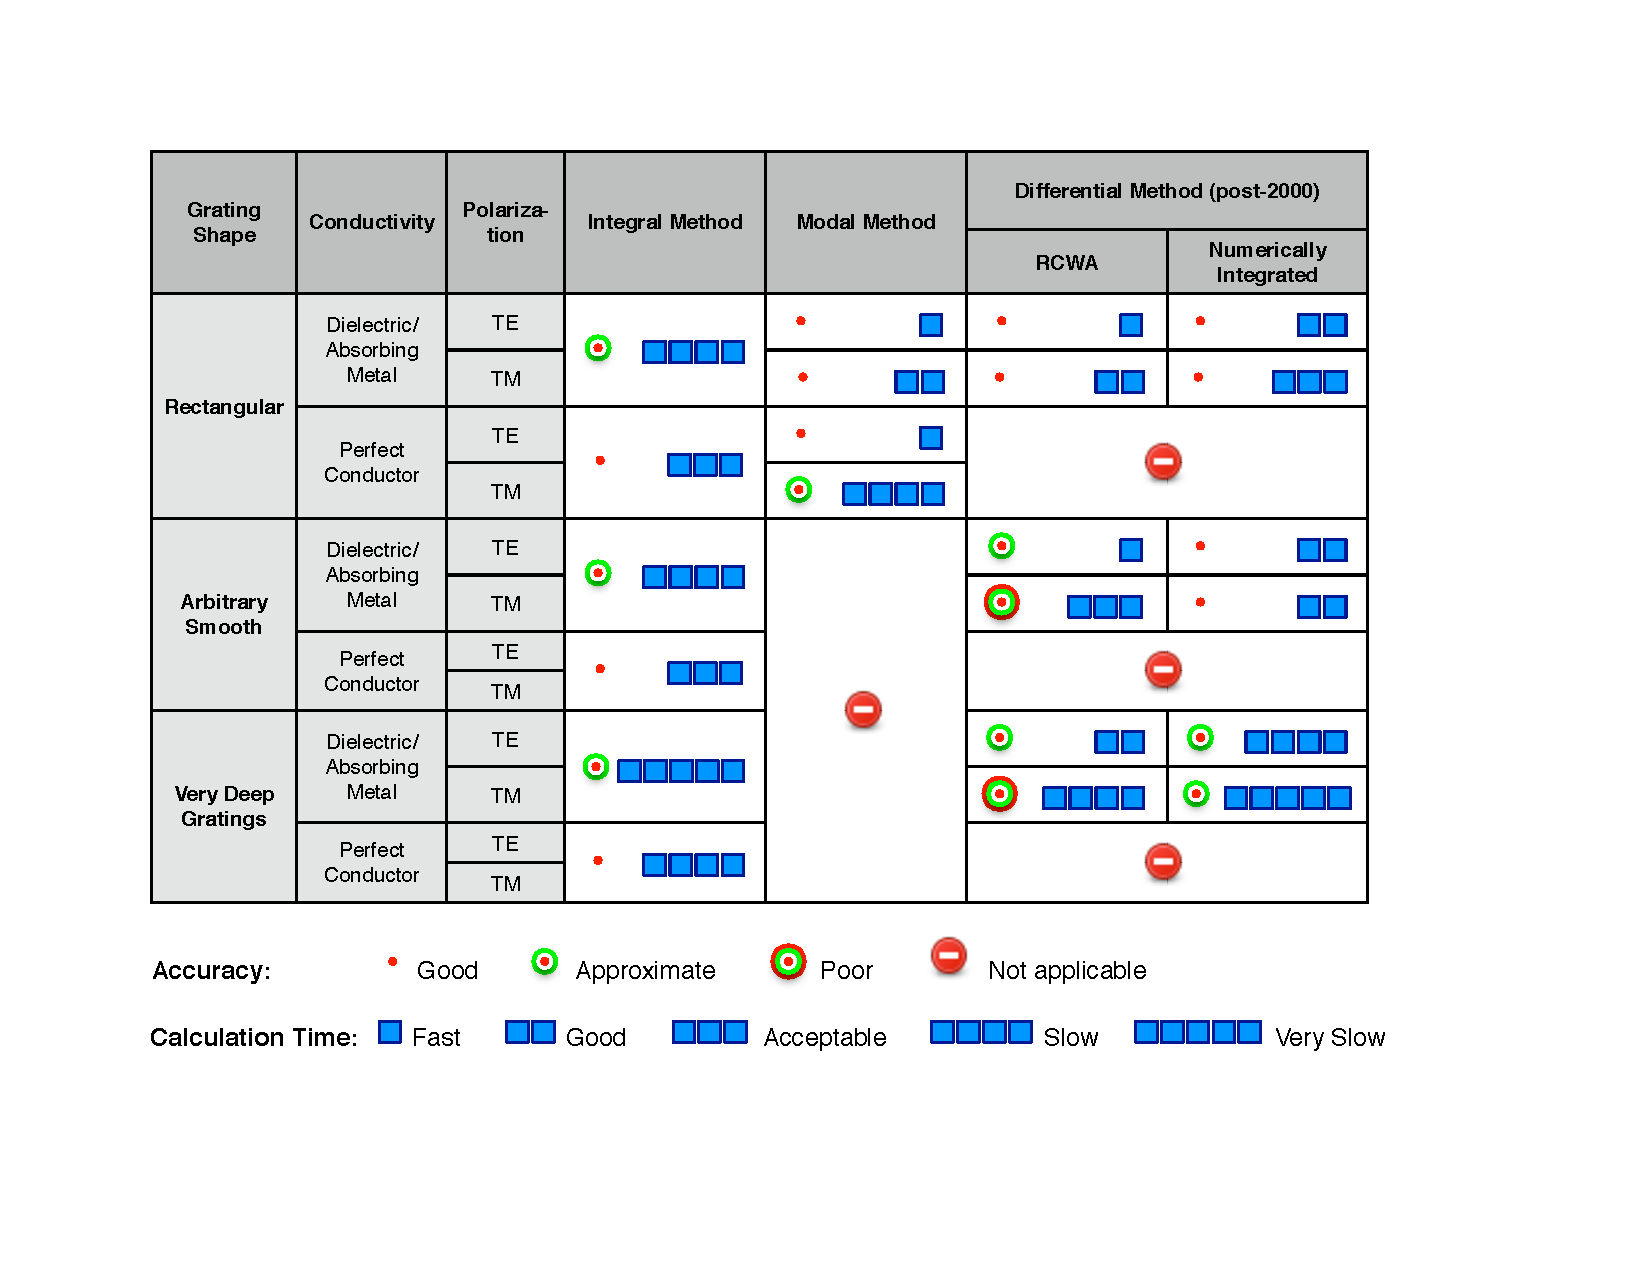
\includegraphics[scale=0.8]{../data/Chapter2/2e_methodComparision/methodComparisonTable_noPre2000.pdf} 
   \caption[A visual comparison of the limitations and strengths of the main methods in grating theory.]{A visual comparison of the limitations and strengths of the main methods in grating theory: the integral approach, the modal method, the full (numerically integrated) differential method, and the differential method's ``RCW'' staircase-approximation simplification.}
   \label{2e}
\end{figure}
 

\subsubsection{Choosing a theoretical method}
Since we are primarily interested in the efficiency of soft x-ray gratings used in grazing incidence, the limitations identified above provide clear guidance for choosing an appropriate method.  At the frequency of soft x-ray radiation, metals behave as absorbing, weak dielectrics with a refractive index near $(0.999 - 0.001i)$; therefore, we do not need to worry about limitations on perfectly-conducting materials.  At grazing incidence, polarization effects are also minimized; there turns out to be very little difference between measured and calculated results for TE and TM polarization.

However, we must be able to model a variety of groove profiles, including rectangular, triangular, trapezoidal, and sinusoidal shapes, with at least one coating layer.  (The triangular, or ``blazed'' profile -- featuring sharp vertices -- turns out to be particularly important for our spectrometer design.)  Therefore, we ruled out the modal and RCW methods, and were left with a choice between the integral method and the full differential method.    Given the necessity of modelling coatings and sharp profiles, we selected the differential method for its simplicity and robustness.  We used two implementations of this method for all the grating efficiency calculations, optimizations, and comparisons shown later in this thesis.

\subsection{Overview of the differential theory}
\label{overview}
The rest of this chapter lays the groundwork for a full electromagnetic theory describing the interaction of light waves with periodic structures.  The conventions we use here are applicable to either the classical differential or RCW methods, and the notation is consistent with the notation used by Neviere in \cite{Nev02}.  However, before diving into the details of the mathematics, it might be useful to summarize the basic physical principles behind the solution:
  \begin{enumerate}
\item The theory starts by using the Maxwell equations to derive a 2nd-order wave equation for the electric and magnetic field of the light.  According to classical optics, the incoming light can be divided into two independent polarization components; the ``Transverse Electric'' (TE) component has its \emph{electric} field vector always parallel to the $z-$axis in Figure \ref{2a}, and the ``Transverse Magnetic'' (TM) component has its \emph{magnetic} field vector always parallel to the $z-$axis.  Due to the beautiful symmetry of the Maxwell equations, it turns out that the wave equation for the electric field in TE polarization is the same as the equation for the magnetic field in TM polarization, and for most of the theory we can use the same mathematics to work with both, referred to as the ``general field'' or just ``the field''.\footnote{While the wave equation is the same for both the TE electric field and the TM magnetic field, the boundary conditions for the fields at the grating interface are different and need to be handled separately.  This is responsible for the difference in efficiency dependent on polarization.}  Because the TE and TM polarizations are independent, we can solve the grating problem for both separately, and then combine the diffracted field solutions in proportion to the polarization of the incident light.
\item Because the grating is periodic, we use Fourier series expansions in the horizontal direction to express both the permittivity of the grating material, and the field itself. In the vertical direction, there are three distinct regions:
	\begin{itemize}
	\item Region 2: above the grooves, where the refractive index is uniform ($\nu = \nu_2$);
	\item Inside the grooves -- the ``modulated region'' -- where the refractive index changes as a function of the $x$ and $y$ position: it is either $\nu_1$ or $\nu_2$;
	\item Region 1: below the grooves, inside the grating substrate, where the refractive index is again uniform ($\nu=\nu_1$).
	\end{itemize}
\item \textbf{Above and below the grooves:}\\
By using the grating as a periodic operator and applying boundary conditions for the field at infinite, we can prove that light is reflected and transmitted at discrete angles, and that a sum of plane waves known as the Rayleigh Expansion can be used to express the total field that satisfies the wave equation in this region.  Each propagating plane wave corresponds to a diffraction ``order'', and once we know the angle of the incident light, we can determine the angles of the diffraction orders (Figure \ref{2b}).  At this point, the Rayleigh expansion still has unknown coefficients, and we need to determine these coefficients to find out how much energy is diffracted into each order.
\item \textbf{Within the grooves:}\\
However, the field within the grooves depends on the exact shape of the groove profile and the interaction of light within the material.  It cannot be simply represented as a sum of plane waves, and the boundary conditions are complicated.  There are two leading methods used to handle this.  Both express the wave equation using Fourier expansions for the field and the grating permittivity.  (These expansions would theoretically be infinite sums, therefore they need to be truncated for computer calculations.  Special rules apply for accurately calculating the products  of truncated Fourier series when they have discontinuities -- for example, the normal component of the electric field at the grating boundary; these were discovered by Li in Reference \cite{Li96b}.)
\begin{enumerate} 
	\item In the ``Rigorous Coupled Wave'' (RCW) approach \cite{Moh81} \cite{Moh95}, the grating groove shape is sliced into thin layers (Figure \ref{3a}) and approximated with vertical walls between layers (the ``staircase approximation'').  This simplifies the boundary conditions because the normal and tangential field components are either entirely along the $x$- or $y$-axis; thus, at every layer the boundary value problem can be converted into a set of simultaneous linear equations and solved algebraically.  Each layer is treated as a separate grating, and the effects of each layer on the up-going and down-going fields are propagated to the next using matrix methods.  (As we describe in Section \ref{methodComparison}, the RCW accuracy and convergence suffers in TM polarization because the staircase approximation introduces sharp corners and artificially large electric field components at the step boundaries \cite{Pop02}.)
	
%	This approach is computationally efficient, and has been known to work accurately in TE polarization.  However, in TM polarization, the results often do not match experimental measurements, because the staircase approximation introduces sharp corners and artificially large electric field components at the step boundaries  \cite{Pop02}.  These sharp corners also demand a higher number of Fourier coefficients to represent the field satisfactorily.
	\item In the ``Differential Method'' approach \cite{Pop00}, we numerically integrate the wave equation many times using different assumed initial values, to generate a complete orthogonal set of particular solutions. Then we use techniques of linear algebra to solve for the coefficients of the general solution that satisfy the boundary conditions along the grating interface.
	\end{enumerate}
\item Finally, most common grating structures consist of one (or often many) stacked layers.\footnote{For example, dielectric gratings with a metal coating used for soft x-ray beamlines, gratings with thin-film multilayer coatings, etc.} (Typical and contrived examples are shown in Figures \ref{2d-1} and \ref{2d-2}).  In classical optics, the \emph{reflection matrix} and \emph{transmission matrix} are often used to propagate an incoming field through an optical layer.  We can generalize this concept to gratings by defining a matrix that maps the Rayleigh coefficients of the incident field to the coefficients of the field that is reflected and transmitted by each layer.  The matrices for each layer can then be multiplied together to find the effect of the complete grating; this is known as the ``T-matrix'' approach.  While theoretically sound, the T-matrix becomes unstable in computer calculations because rounding errors introduce instability into growing exponential functions.  An alternative formulation called the ``S-matrix'' approach defines a matrix at each layer that represents the cumulative effect of \emph{all layers below and including that layer} on the incident field; by definition, this matrix remains bounded and is safe to use for numerical calculations \cite{Li96}.  This matrix links the Rayleigh coefficients of the up-going and down-going waves between each layer with the more complicated functions within the grooves of each layer, where the Rayleigh expansion does not apply. 
\end{enumerate}

\label{stacksOfGratings}
\begin{figure}[p] %  figure placement: here, top, bottom, or page
   \centering
   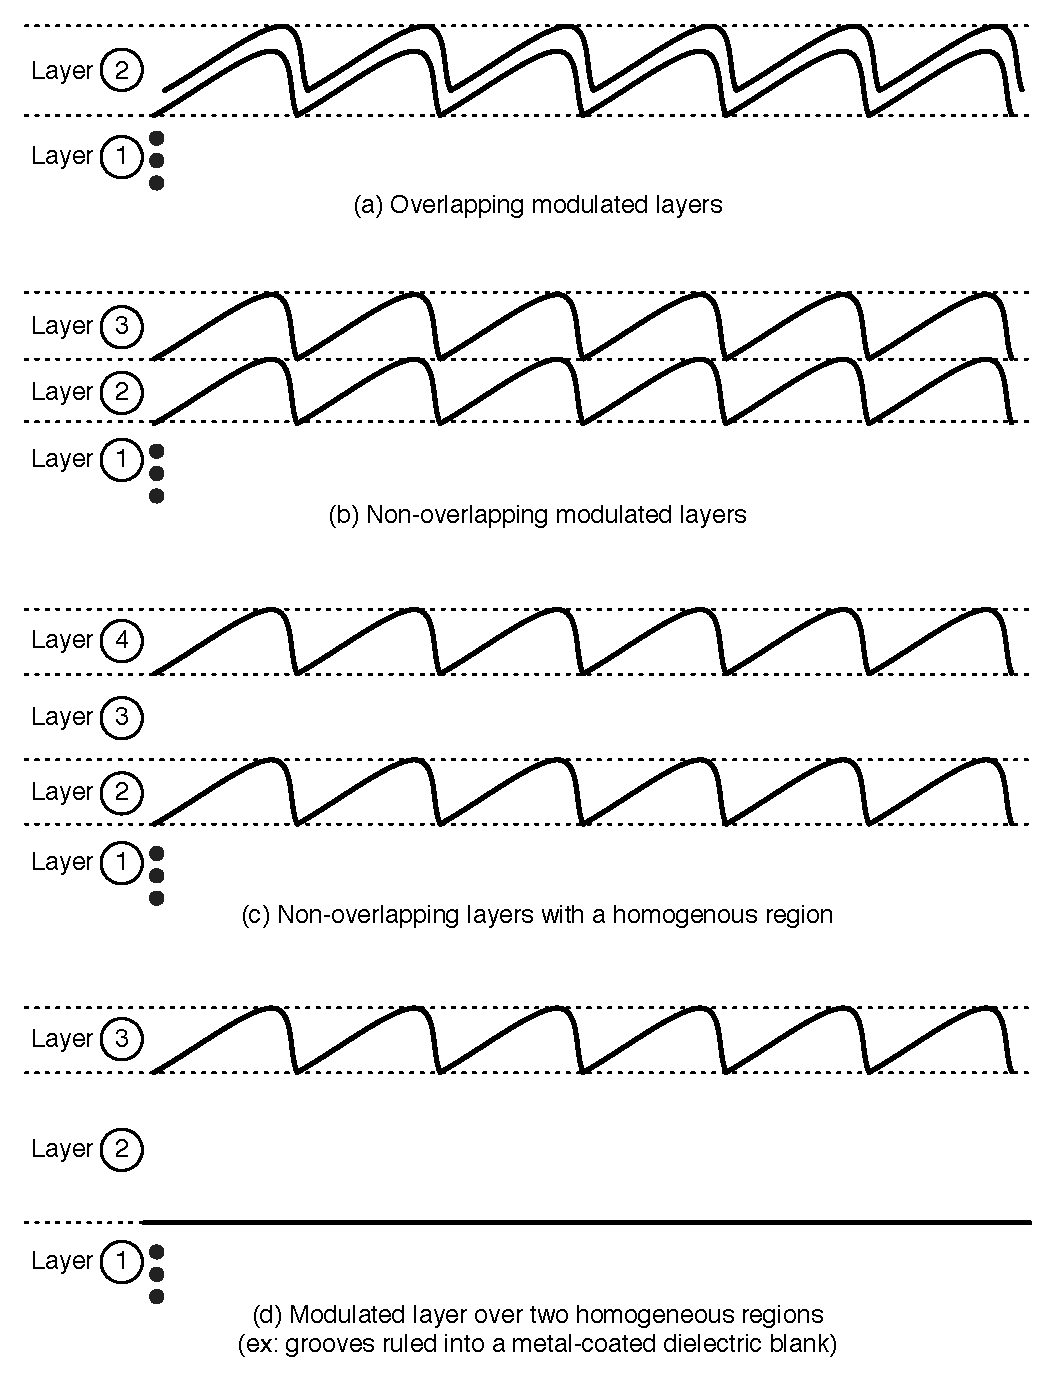
\includegraphics[scale=0.5]{../data/Chapter2/2d_stacksOfGratings/2d_1.pdf} 
   \caption{Arbitrarily-complicated structures can be handled by dividing the grating into layers, where each layer is either homogenous (constant refractive index), or modulated (with a refractive index that changes periodically as a function of $x$ at any given height $y$).}
   \label{2d-1}
\end{figure}

\begin{figure}[p] %  figure placement: here, top, bottom, or page
   \centering
   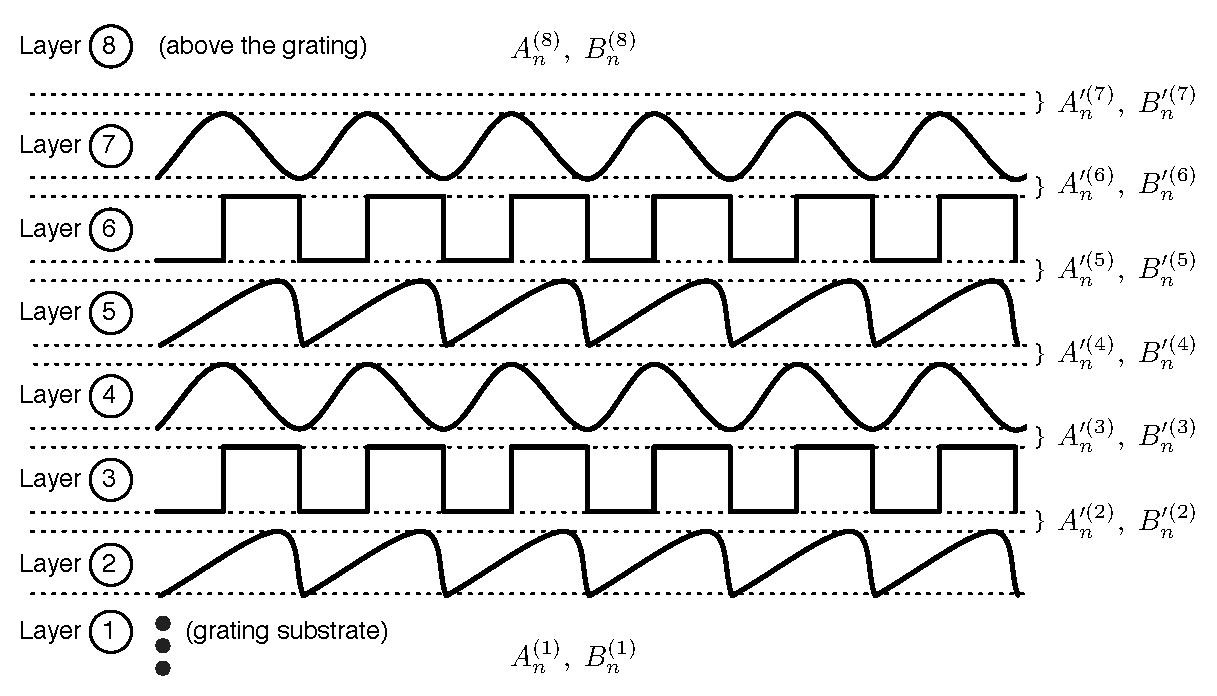
\includegraphics[scale=0.5]{../data/Chapter2/2d_stacksOfGratings/2d_2.pdf} 
   \caption[Modulated layers in a complicated stack of gratings.  In between every layer, we can insert an imaginary, infinitely-thin homogenous layer where the Rayleigh expansion applies.]{Modulated layers in a complicated stack of gratings.  In between every layer, we can insert an imaginary, infinitely-thin homogenous layer where the Rayleigh expansion applies.  The $A^{\prime}_n$ and $B^{\prime}_n$ expansion coefficients connect the boundary conditions between layers.  Within each layer, the Rayleigh expansion does not apply -- inside the grooves, the field cannot be represented as a simple sum of plane waves -- and numerical methods are required to approximate it.}
   \label{2d-2}
\end{figure}

\subsection{Simplifying assumptions}
\label{s_assumptions}
Before we tackle the mathematics of grating theory, this section defines the geometry and terminology we use throughout the text, and introduces some assumptions that simplify the problem.  Figure \ref{2a} shows a side view of a reflection grating, in the following situation:
\begin{enumerate}
\item The mean surface of the grating is in the $x-z$ plane, with the grooves running parallel to the $z-$axis.  The groove profile is periodic and repeats every distance $d$ along the $x-$axis.
\item The grating is described by the profile function $y_p = g(x)$, which has a minimum of $y=0$, a maximum $y=a$, and is periodic on $d$:
\begin{align}
y_p = g(x) = g(x+d)
\end{align}
\item The grating is illuminated with a light ray travelling parallel to the $x-y$ plane (i.e.: within the plane of the page). This is referred to as ``in-plane incidence'', and is typical of how most monochromators and spectrometers are used.  (When the incident ray has a component in the $z-$direction, the diffraction peaks end up dispersed over the surface of a three-dimensional cone, and this is referred to as ``conical mounting''.)
\end{enumerate}
These first two simplifications reduce the grating problem to two dimensions, since the whole system is unchanged by translation along the $z-$axis.

Additionally, we assume that:
\begin{enumerate}
\item The incident light can be represented as a plane wave, infinite in extent.  
\item The grating also stretches forever in the $x-$ and $z-$directions.

\end{enumerate}
Typical gratings used in soft x-ray devices are much much larger (typically: 40 mm) than their groove spacing $d$ (typically: a few $\mu$m).  As long as they are illuminated with collimated light having a beam width much larger than the groove spacing, both of these assumptions seem reasonable.

Finally, to simplify the electromagnetic field calculations, we assume that
\begin{enumerate}
\item The grating material is non-magnetic, with a permeability of $\mu_0$.
\item The dielectric constant $\epsilon$ of the grating material is the same in all directions.
\end{enumerate}
(These last two assumptions are also necessary to keep us within a two-dimensional problem.  If the material is non-isotropic, then the dielectric constant $\epsilon$ becomes a tensor $\left[\left[\epsilon\right]\right]$ and the problem requires a full 3D analysis.)

These assumptions make the grating theory much simpler to present in this chapter. However, it should be noted that at the expense of larger matrices and higher mathematical complexity, it is possible to express the same theory in the full three-dimensional case, which enables the analysis of exotic situations like conical mount gratings, crossed 2D gratings, and non-isotropic materials.  Reference \cite[Chapter 5]{Nev02} provides a derivation of the full 3D version.

We assume that the grating surface exactly matches the periodic profile given by $y_p=g(x)$ in Figure \ref{2a}.  For real-world applications, this turns out to be the most unfounded assumption, since actual gratings vary from groove to groove due imperfections in the manufacturing process, and their ideally smooth surfaces have an unavoidable amount of random roughness.  Unfortunately, this assumption is necessary for any mathematical treatment; in Section \ref{realWorldEffects}, we look at the impacts of real-world  imperfections on grating efficiency.

\subsubsection{A few notes on notation:}
\begin{itemize}
\item Quantities that change depending on the grating region are subscripted to indicate the region they are in.  For example, $k_2$ and $\nu_2$ designate the wave vector and refractive index, and $\theta_{2,n}$ the angle of the $n$-th order ray, in Region 2 above the grating.  Eventually, we tackle layered gratings with many numbered regions, and this subscript convention becomes helpful.
\item Angles are measured from the surface normal as shown in Figure \ref{2a}.  There are two different sign conventions in common use; we use positive angles for both the incident ray ($\theta_2$) and the diffracted ray ($\theta_{2,n}$) when they are on opposite sides of the surface normal.  Transmitted rays ($\theta_{1,n}$) are also measured using positive angles from the $-y$ axis, as shown in Figure \ref{2a}.\footnote{The sign convention for diffraction angles affects the sign in the right-hand side of the grating equation \eq{gratingEquation}.  In North American literature it is more common to measure all angles positive counter-clockwise from the surface normal; this creates a `$+$' rather than a `$-$' in the grating equation.}
\end{itemize}

\subsection{Electromagnetic field and polarization}
In Figure \ref{2a}, incoming light strikes the grating along wavevector $\vec k_2$ at an angle $\theta_2$ from perpendicular to the grating plane.
\begin{align}
\vec k_2 &= \nu_2 \frac{\omega}{c} \left( \sin \theta_2 \vec{\hat x} - \cos \theta_2 \vec{\hat y} + 0 \vec{\hat z} \right)
\end{align}
We use $\nu$ to designative the refractive index. Here, $\nu_2$ designates the refractive index in Region 2 above the grating, which is normally air or vacuum.  (In Region 1, the grating material might be absorbing, which means the material's refractive index $\nu_1$ would have an imaginary component greater than 0.)  Frequency $\omega = 2\pi f$ is the angular frequency of the light, and $c$ is the speed of light in vacuum.

The incoming light is a travelling electromagnetic plane wave with sinusoidal dependence on time.  We can express the electric field vector using the complex exponential form:
\begin{align}
\label{eqnPlaneWave}
\vec E_{incident} &= \vec A\, \exp \left(i (\vec k_2 \,  \vec r - \omega t)\right)  = \vec A\, \exp \left(i\, k_2 (x \sin \theta_2 - y \cos \theta_2)\right)\exp \left(- i \omega t\right)
\end{align}
where the true (physical) field is contained in the real part.  Since all fields will have the same harmonic dependence on time, we drop the $e^{-i\omega t}$ factor from here on.  (The scalar $k_2$ is simply the magnitude of $\vec k_2$, i.e.: $\left| \vec k_2 \right| = \nu_2\, \omega/c$.)

The electric field vector is always perpendicular to the direction of the wave $\vec k_2$, but can have an arbitrary polarization determined by $\vec A$.  This can always be expressed as a superposition of two orthogonal components:
\begin{itemize}
\item The TE (transverse electric) polarization represents the component of the electric field vector parallel to the $z$ axis (i.e.: into the page).  For a pure TE wave, the $E_x$, $E_y$, and $B_z$ fields are always 0.
\item The TM (transverse magnetic) polarization represents the component of the electric field vector in the $x-y$ plane (i.e.: the \emph{magnetic} field vector is along $z$).  For a pure TM wave, the $E_z$, $B_x$, and $B_y$ fields are always zero.
\end{itemize}
In general, the grating problem is solved by applying the Maxwell equations to the incident electric field, according to the boundary conditions imposed by the grating.  By solving it separately for each polarization case (TE and TM), we can simplify these equations.  In the end, we superpose the results calculated for the outgoing fields, weighted by the actual polarization of the incident light.

\subsection{Maxwell's equations for sinusoidal time-varying fields}
Our assumptions in Section \ref{s_assumptions} mean that the gratings are not loaded with free charge, or carrying free currents. Therefore, the two relevant Maxwell equations are:
\begin{align}
\nabla \times \vec E &= - \frac {\partial \vec B }{\partial t}
\end{align}
\begin{align}
\nabla \times \vec B &= \mu \epsilon \frac{ \partial \vec E }{ \partial t }
\end{align}
For sinusoidal time-varying fields, the electric field $\vec E$ is proportional to $e^{-i \omega t}$, so the time derivatives reduce to:
\begin{align}
\nabla \times \vec E &= i \omega \mu \vec H
\end{align}
\begin{align}
\nabla \times \vec H &= - i \omega \epsilon \vec E
\end{align}
or, expressed in Cartesian coordinates:
\begin{align}
\label{maxwellEqn1}
\frac{\partial E_z}{\partial y} - \frac{\partial E_y}{\partial z} &= i \omega \mu H_x  \\
\label{maxwellEqn2}
\frac{\partial E_x}{\partial z} - \frac{\partial E_z}{\partial x} &= i \omega \mu H_y  \\
\label{maxwellEqn3}
\frac{\partial E_y}{\partial x} - \frac{\partial E_x}{\partial y} &= i \omega \mu H_z  \\
\label{maxwellEqn4}
\frac{\partial H_z}{\partial y} - \frac{\partial H_y}{\partial z} &= -i \omega \epsilon E_x  \\
\label{maxwellEqn5}
\frac{\partial H_x}{\partial z} - \frac{\partial H_z}{\partial x} &= -i \omega \epsilon E_y \\
\label{maxwellEqn6}
\frac{\partial H_y}{\partial x} - \frac{\partial H_x}{\partial y} &= -i \omega \epsilon E_z
\end{align}
Since the grating and the incident light are uniform along the $z-$axis, all of the partial derivatives with respect to $z$ are 0.  For TE polarization, since $E_x$ and $H_z$ are 0, equations \eq{maxwellEqn1}, \eq{maxwellEqn2}, and \eq{maxwellEqn6} are decoupled into
\begin{align}
\frac{\partial E_z}{\partial y} &= i \omega \mu H_x
\label{mete1}
\end{align}
\begin{align}
-\frac{\partial E_z}{\partial x} &= i \omega \mu H_y
\label{mete2}
\end{align}
and
\begin{align}
\frac{\partial H_y}{\partial x} - \frac{\partial H_x}{\partial y} &= - i \omega \epsilon E_z
\label{mete3}
\end{align}
We can use \eq{mete1} and \eq{mete2} to eliminate $H_x$ and $H_y$ in \eq{mete3}:
\begin{align}
\frac{i}{\omega \mu} \frac{\partial^2 E_z}{\partial x^2} + \frac{i}{\omega \mu}  \frac{\partial^2 E_z}{\partial y^2} &= -i \omega \epsilon E_z
\label{mete4}
\end{align}
Note that $\epsilon$ is a function of position $\epsilon(x,y)$, since it changes whether inside the grating or above the grating.  Since 
\begin{align}
k^2(x, y) = v^2(x,y)\, \omega^2/c^2 = \omega^2 \mu \epsilon(x, y),
\end{align}
we get a single second-order wave equation in $E_z$:
\begin{align}
\nabla^2 E_z + k^2 E_z = 0,
\label{wete}
\end{align}
where $E_z = E_z(x,y)$ and $k^2 = k^2(x,y)$ are both functions of position.


For the case of TM polarization, the Maxwell equations \eq{maxwellEqn4}, \eq{maxwellEqn5}, and \eq{maxwellEqn3} reduce to 
\begin{align}
\frac{\partial H_z}{\partial y} &= -i \omega \epsilon E_x \\
-\frac{\partial H_z}{\partial x} &= -i \omega \epsilon E_y \\
\frac{\partial E_y}{\partial x} - \frac{\partial E_x}{\partial y} &= i \omega \mu H_z
\end{align}
and an identical procedure produces the wave equation in $H_z$:
\begin{align}
\label{wetm}
\nabla\left[  \frac{1}{k^2} \nabla H_z  \right] + H_z &= 0% \\
%\nabla^2 H_z + k^2 H_z &= 0
\end{align}
In general, $k$ here is still a function of position $k(x,y)$ depending on whether we are inside or outside of a groove valley, or above or below the modulated region.  However, in the homogenous space above and below the modulated region, $k$ is constant and both \eq{wete} and \eq{wetm} reduce to the Helmholtz equation:
\begin{align}
\nabla^2 U_z + k^2 U_z &= 0
\end{align}
Due to the (near) symmetry of the Maxwell equations, the form of the wave equation in homogeneous space is the same for the $U_z = H_z$ field in TM polarization as it is for the $U_z = E_z$ field in TE polarization.  To solve the grating problem, we need to find the solution to this wave equation in the presence of the grating boundary conditions.\footnote{Although the wave equation is the same, the boundary conditions for electric and magnetic fields are different at the grating boundary where $\epsilon$ and $v$ change suddenly -- for example, the normal component of the electric field is discontinuous, while the normal component of the magnetic field is continuous. This leads to a difference in the TE and TM efficiency.}
\subsection{Periodicity of gratings and fields (aka, pseudo-periodic functions and the Fourier basis)}
The periodic nature of the grating grooves immediately hints that we could represent them conveniently using a Fourier series.  But can a Fourier expansion also be used to represent the fields $E_z$ and $H_z$?

Here we define $u = E_z$ when working in TE polarization, and $u = H_z$ when working in TM polarization; it represents the ``generic field''.  The grating can be imagined as an operator $\mathbb{G}$ that transforms the incident field $u_i$ into a diffracted field $u$:
\begin{align}
u(x,y) = \mathbb{G} \, u_i(x,y)
\end{align}
Because the grating is periodic and extends forever, the operator $\mathbb{G}$ is invariant (does not change) under translation by a grating period: $x \rightarrow x+d$.  
\begin{align}
u(x+d,y) = \mathbb{G} \, u_i(x+d,y)
\end{align}
Since the incident light arrives at an angle $\theta_2$, this translation adds an extra path distance $d \sin \theta_2$ to the incident wave $u_i$, for a phase change $e^{i k_2 d \sin \theta_2}$:
\begin{align}
u_i(x+d, y) = e^{i k_2 d \sin \theta_2} u_i(x, y) = C \, u_i(x,y)
\end{align}
where the constant $C$ has been matched to $e^{i k_2 d \sin \theta_2}$.

Because the set of coupled Maxwell partial differential equations \eq{maxwellEqn1} to \eq{maxwellEqn6} is linear, any solution multiplied by a constant $C$ is still a solution:
\begin{align}
u(x,y) &= \mathbb{G} \, ( u_i(x,y) \, ) \\
C \, u(x,y) &= \mathbb{G} \, ( C \, u_i(x,y) \, ) \\
C \, u(x, y) &= \mathbb{G} \, u_i(x+d,y)
\end{align}
but since $\mathbb{G} \, u_i(x+d,y) = u(x+d, y)$ also,
\begin{align}
C \, u(x, y) &= u(x+d, y)
\end{align}
In other words, the total field translated by one period $d$ is equal to its untranslated self, multiplied by a complex constant:
\begin{align}
u(x+d, y) &= C \, u(x, y) = e^{i k_2 d \sin \theta_2} u(x,y) = e^{i \alpha_0 d} u(x,y)
\end{align}
where we have defined 
\begin{align}
\boxed{\alpha_0 \equiv k_2 \sin \theta_2}
\end{align}
This is known as a \emph{pseudo-periodic} relationship:
\begin{align}
u(x+d, y) &= e^{i \alpha_0 d} u(x,y)
\end{align}
since a true (strictly) periodic relationship would have the form:
\begin{align}
v(x+d, y) &= v(x,y)
\end{align}
However, we can easily create such a function by defining $v \equiv e^{-i \alpha_0 x} u$.  As a legitimately periodic function, $v$ can be represented as a Fourier series expansion on the grating period $d$:
\begin{align}
v(x, y) &= e^{-i \alpha_0 x} u(x,y) \\
v(x,y) &= \sum_{n=-\infty}^{\infty} u_n(y) e^{i2\pi n x/d} \\
u(x,y) &= e^{i \alpha_0 x} \sum_{n=-\infty}^{\infty} u_n(y) e^{i2\pi n x/d}
\end{align}
If we define 
\begin{align}
\boxed{\alpha_n \equiv \alpha_0 + 2 \pi n / d}
\end{align}
we can express the total field as something that looks \emph{very close} to a Fourier series expansion:
\begin{align}
\label{eqnFourierExpansionU}
u(x,y) &=  \sum_{n=-\infty}^{\infty} u_n(y) e^{i\alpha_nx}
\end{align}
This is the Fourier basis for the total field $u = E_z$ or $H_z$, with an infinite number of Fourier coefficients $u_n$.  (Eventually, we will need to truncate this series to work with it numerically.)
\subsection{Deriving the Grating Equation}
Equipped with a Fourier expansion for the total field and a wave equation, we can attempt to solve for the field.  Figure \ref{2a} shows the coordinate system sliced into three regions: 
\begin{itemize}
\item Region 2: Above the grooves where $y>a$, the impedance $k(x, y)$ is constant and proportional to the refractive index of the air/vacuum: $k_2(x, y)=v_2 \omega/c$.
\item Region 1: Below the grooves where $y<0$, the impedance $k(x,y)$ is also constant and proportional to the grating's refractive index: $k_1(x,y)=v_1 \omega /c$.
\item Inside the grooves, the impedance is changing as a function of position: whether inside or outside of a groove.  We ignore this difficult region for now and try to work with the uniform regions as much as possible.
\end{itemize}
Where $k(x,y)$ is constant, the wave equations for both TE \eq{wete} and TM polarization \eq{wetm} reduce to:
\begin{align}
\nabla^2 u + k^2 u = 0
\end{align}
where $k=k_1$ above the grating, and $k=k_2$ below it.  If we insert the Fourier expansion for the field $u(x,y)=\sum u_n(y) e^{i\alpha_n x}$ into the wave equation:
\begin{align}
\nabla^2 \left( \sum_{n=-\infty}^{\infty} u_n(y) e^{i2\pi nx/d}e^{i\alpha_0 x} \right) + k^2 \sum_{n=-\infty}^{\infty} u_n(y) e^{i2\pi n x/d}e^{i\alpha_0 x} &= 0 \\
e^{i \alpha_0 x} \sum_{n=-\infty}^{\infty}  \left( \frac{\partial^2}{\partial y^2} + (k^2 - (\alpha_0+2\pi n/d)^2) \right) u_n(y) e^{i2\pi n x/d} &= 0
\end{align}
For this Fourier sum to be equal to zero, all of the coefficients must be zero:
\begin{align}
\left( \frac{\partial^2}{\partial y^2} + (k^2 - (\alpha_0+2\pi n/d)^2) \right) u_n(y) &= 0\\
\left( \frac{\partial^2}{\partial y^2} + (k^2 - \alpha_n^2) \right) u_n(y) &= 0
\end{align}
This is a standard differential equation with the solution
\begin{align}
u_n(y) = A_n e^{-i\beta_n y}+ B_n e^{i\beta_n y}
\end{align}
where 
\begin{align}
\beta_n = \sqrt{k^2 - \alpha_n^2}
\end{align}
and $A_n$ and $B_n$ are unknown constants to be determined by the boundary conditions.

Special attention must be paid to the square root for $\beta_n$, depending on whether we are above or below the grating.

\subsubsection{Above the grating}
  Above the grating, we are likely inside air or vacuum ($k=k_2$), so the refractive index and $k$ would be real.  Since $\alpha_n = \alpha_0 + 2\pi n/d$ increases with $n$, there is a finite number of $n$ near $n=0$ where $(k^2 - \alpha_n^2)$ is a positive number.  However, there are also an infinite number of $n$ (approaching $n\rightarrow \infty$ and $n\rightarrow -\infty$) where $(k_2 - \alpha_n^2) < 0$.  This creates two possibilities for $\beta_n$ (that we label $\beta^{(2)}_n$ because we are in Region 2):
\begin{align}
\beta^{(2)}_n = \sqrt{k^2 - \alpha_n^2} \;\;\;\; & (k^2-\alpha_n^2)>0 \;\;\;\; &\textrm{(finite occurrences, } \beta^{(2)}_n\textrm{ real)} \\
\beta^{(2)}_n = i\sqrt{\alpha_n^2 - k^2} \;\;\;\; & (k^2-\alpha_n^2)<0 \;\;\;\; &\textrm{(infinite occurrences, } \beta^{(2)}_n\textrm{ complex)}
\end{align}
Using this solution for the Fourier coefficients $u_n$, the total field is:
\begin{align}
u(x,y) =  \sum_{n=-\infty}^{\infty} A^{(2)}_n e^{i \alpha_n x - i \beta^{(2)}_n y} +  \sum_{n=-\infty}^{\infty} B^{(2)}_n e^{i \alpha_n x + i \beta^{(2)}_n y}
\end{align}
This result is remarkable.  The total field created above the grating is a finite sum of propagating plane waves (for all $n$ where $\beta^{(2)}_n$ is real) and an infinite sum of decaying (when $\beta^{(2)}_n$ is complex) plane waves.

To expand on this conclusion: The first sum (with $A^{(2)}_n$ coefficients) are waves travelling in the $-y$ direction, down toward the grating.  For the finite set of $n$ where $\beta^{(2)}_n$ is real, these are non-decaying, normal waves.  There is also  an infinite number of exponentially growing waves that explode as $y\rightarrow +\infty$, for the remaining $n$ that cause $\beta^{(2)}_n$ to be complex.

Similarly, the second sum (with $B^{(2)}_n$ coefficients) represents waves travelling away from the grating, in the $+y$ direction.  There is a finite set of propagating waves, and an infinite set of exponentially decaying waves (``\emph{evanescent waves}'') that tend to zero as $y \rightarrow +\infty$.  

\begin{figure}[htbp] %  figure placement: here, top, bottom, or page
   \centering
   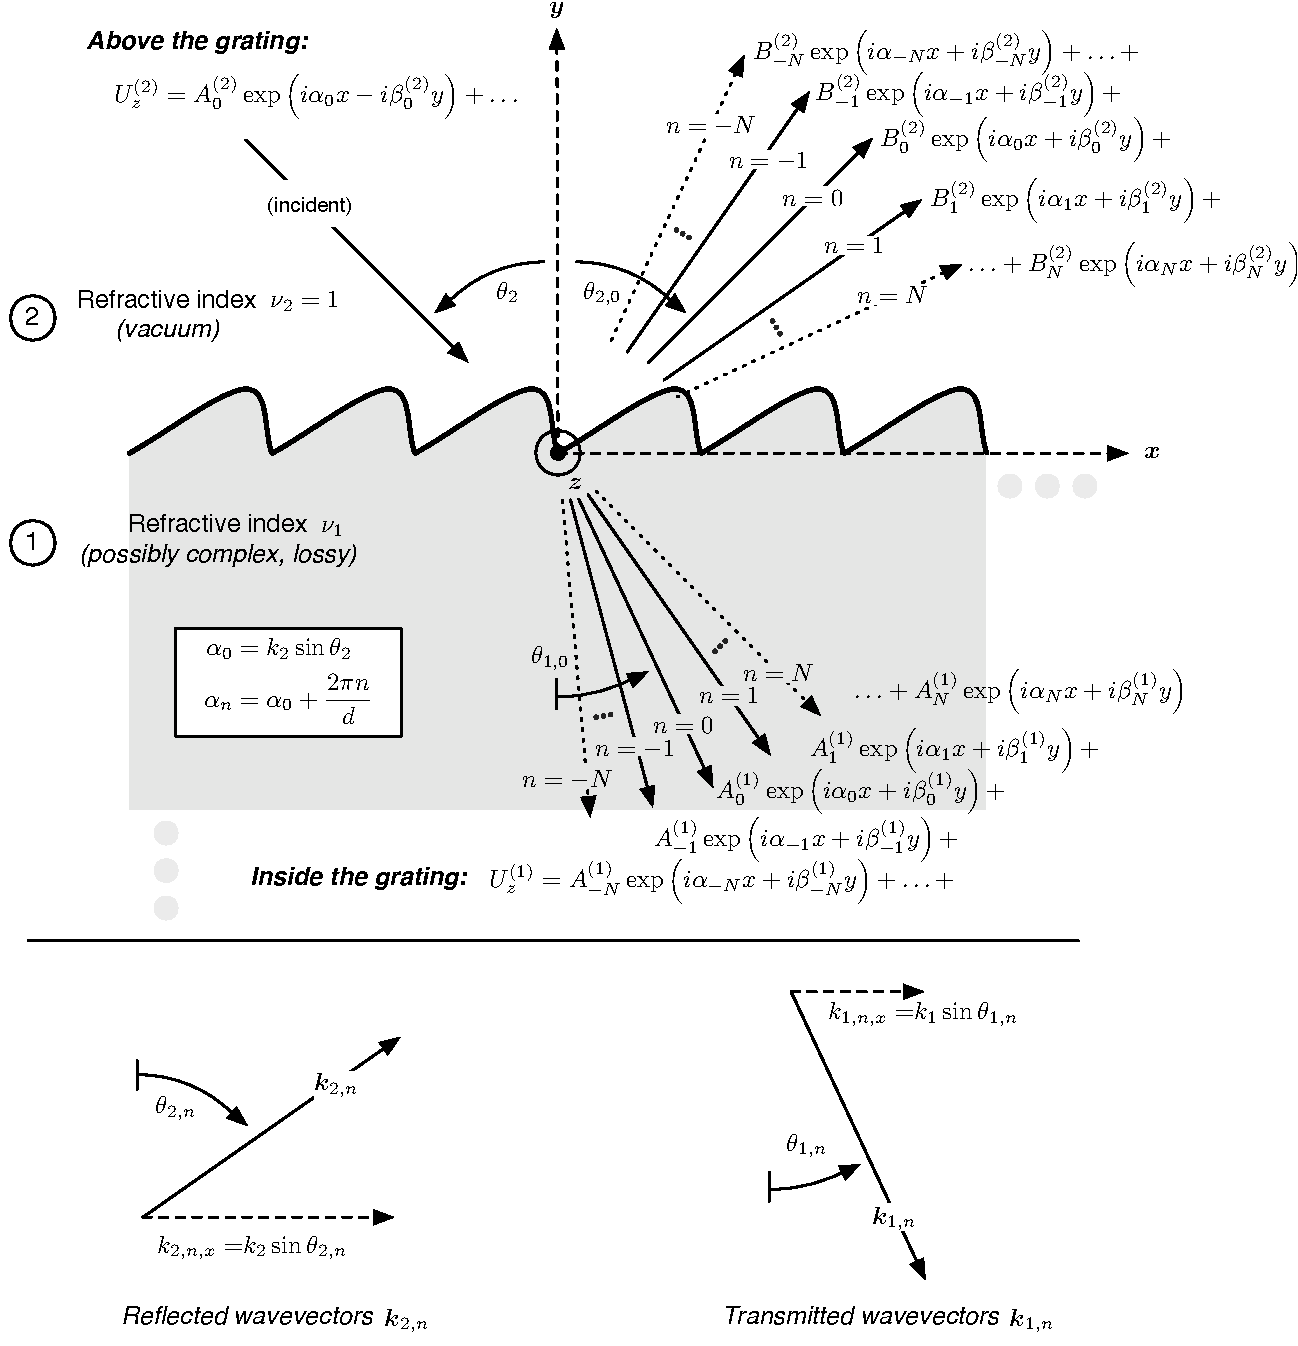
\includegraphics[scale=0.8]{../data/Chapter2/2b_rayleighExpansion/2b.pdf} 
   \caption[The Rayleigh expansion describes the electric field (TE polarization) or magnetic field (TM polarization) in homogenous media, above and below the grating.]{The Rayleigh expansion describes the electric field (TE polarization) or magnetic field (TM polarization) in homogenous media, above and below the grating.  The terms in the expansion include a finite number of propagating plane waves -- the diffraction orders -- and an infinite number of decaying, or ``evanescent'' plane waves. From the geometry of the diffracted and transmitted wave vectors, we can derive the grating equation, but we need to solve the $A_n$ and $B_n$ coefficients to determine the efficiency of each order. }
   \label{2b}
\end{figure}

The total field has a unique solution only when the incident field $u_i$ is totally specified.  From the grating setup in Figure \ref{2a}, we know that we only have a single down-going wave, corresponding to the incident plane wave; all of the $A^{(2)}_n$ for the other propagating waves must be 0.  (We label this incident wave with $n=0$.)  We also need to reject the non-physical waves that explode as $y \rightarrow +\infty$, therefore the expansion of the field \emph{above the grating} simplifies to:
\begin{align}
u(x,y) =  A^{(2)}_0 e^{i \alpha_0 x - i \beta^{(2)}_0 y} +  \sum_{n=-\infty}^{\infty} B^{(2)}_n e^{i \alpha_n x + i \beta^{(2)}_n y}
\label{rayleighExp2}
\end{align}
The diffraction grating's reflected orders appear out of this expansion as the finite set of $n$, $\beta^{(2)}_n$, and $B^{(2)}_n$ values that create propagating plane waves travelling away from the grating.  At this point, $n$ can now be properly identified with the \emph{diffraction order}.  This is known as the \emph{Rayleigh Expansion} for the diffraction field.  (Rayleigh assumed this solution, but did not prove it, in Reference \cite{Ray07}.)  Figure \ref{2b} shows this visually and mathematically. 

\subsubsection{Below the grating}
The field below the grating ($y<0$) can be expanded using the same  technique.  One complication is that for grating materials that absorb energy, the refractive index (and hence $k=k_1$) is complex.\footnote{In fact, this is the case for all materials at soft x-ray wavelengths.}  In this situation there are two possibilities for the square root $\beta^{(1)}_n = \sqrt{k_1^2-\alpha_n^2}$.  The correct choice can be made by requiring that the diffracted waves remain bounded when $y\rightarrow -\infty$; this requires choosing the root where $\operatorname{Im}(\beta^{(1)}_n) > 0$.

Applying the same process as above, we determine an expansion for the transmitted field, corresponding to the transmitted orders.  These are also shown visually in Figure \ref{2b}:
\begin{align}
u(x,y) =  \sum_{n=-\infty}^{\infty} A^{(1)}_{n} e^{i \alpha_n x - i \beta^{(1)}_{n} y}
\label{rayleighExp1}
\end{align}

\subsubsection{The grating equations}
These expansions for the reflected and transmitted fields show that as soon as the direction of the incident wavevector is fixed, the outgoing directions of light are determined.  For the \emph{reflected} orders, Equation \eq{rayleighExp2} gives the $x$- and $y$-components of the wavevectors:
\begin{align}
B^{(2)}_n e^{i(k_x x + k_y y)} &= B^{(2)}_n e^{i(\alpha_n x + \beta^{(2)}_n y)} \\
k_x &= \alpha_n \\
  &= \alpha_0 + \frac{ 2\pi n}{d} \\
  &= k_2 \sin \theta_2 +\frac{ 2\pi n}{d}
\end{align}
From the geometry analyzed in Figure \ref{2b}, the $x$-component of the outgoing wavevector at angle $\theta_{2,n}$ is $k_2 \sin \theta_{2,n}$.  Therefore
\begin{align}
\label{kxEqn2}
k_x &= k_2 \sin \theta_2 +\frac{ 2\pi n}{d} = k_2 \sin \theta_{2,n}
\end{align}
and, after replacing the magnitude of the wavevector above the grating $k_2 = \nu_2\, \omega / c = \nu_2 \, 2\pi f / c =  2\pi / \lambda$, the famous grating equation (for reflected orders) is finally:
\begin{align}
\label{gratingEquation}
\frac{n \lambda}{d} = \sin \theta_{2,n} -  \sin \theta_{2}
\end{align}
(where we have assumed that $\nu_2 = 1$ because we are in free space, and $\lambda$ is also the free-space wavelength.) This is often called the \emph{Fraunhofer Grating Equation}.

When $n=0$, the grating equation reverts to the law of reflection ($\theta_{2,0} = \theta_2$, i.e.: the angle of reflection is equal to the angle of incidence.)  This wave corresponds to a classically-reflected wave from a normal surface.  The reflected orders that fall \emph{between} the incident wave and the $n=0$ reflection are referred to as \emph{inside orders}; using our sign convention for diffraction angles, they correspond to $n<0$.  The \emph{outside orders} ($n>0$, see Figure \ref{2b}) are diffracted at angles beyond the $n=0$ reflection.

We can also use the same technique to determine the angles of the transmitted orders.  Equation \eq{rayleighExp1} gives the $x$- and $y$-components of the transmitted wavevectors:
\begin{align}
A^{(1)}_n e^{i(k_x x + k_y y)} &= A^{(1)}_n e^{i(\alpha_n x + \beta^{(1)}_n y)} \\
k_x &= \alpha_n = \alpha_0 + \frac{ 2\pi n}{d} = k_2 \sin \theta_2 +\frac{ 2\pi n}{d}
\end{align}
From the geometry analyzed in Figure \ref{2b}, the $x$-component of the outgoing wavevector at angle $\theta_{1,n}$ is $k_1 \sin \theta_{1,n}$.  Therefore
\begin{align}
\label{kxEqn1}
k_x &= k_2 \sin \theta_2 +\frac{ 2\pi n}{d} = k_1 \sin \theta_{1,n}
\end{align}
and, after again replacing $k_1$, the magnitude of the wavevector below the grating $k_1 = \nu_1\, \omega / c = \nu_1 \, 2\pi f / c =  \nu_1 \, 2\pi / \lambda$, the transmission grating equation is:
\begin{align}
\label{gratingEquation}
\frac{n \lambda}{d} = \nu_1 \, \sin \theta_{1,n} -  \nu_2 \, \sin \theta_{2}
\end{align}
This time, instead of checking for the law of reflection, we can check that when $n=0$, the transmission equation reverts to Snell's law of refraction ($\nu_1\, \sin \theta_{1,0} = \nu_2 \, \sin \theta_2$).

\subsubsection{Note: Simplifying $\beta_n$}
Equations \eq{kxEqn2} and \eq{kxEqn1} provide a useful simplification for $\beta_n$.  Since 
\begin{align}
k_2 \sin \theta_2 +\frac{ 2\pi n}{d} = k_2 \sin \theta_{2,n} = k_1 \sin \theta_{1,n}
\end{align}
we can go back to the expression for $\beta_n$, and easily show that 
\begin{align}
\beta_n^{(2)} &= \sqrt{k_2^2 - \alpha_n^2} = \sqrt{k_2^2 - (\alpha_0 +2\pi n/d)^2} \\
&= \sqrt{k_2^2 - (k_2 \sin \theta_2 +2\pi n/d)^2}\\
&= \sqrt{ k_2^2 - (k_2 \sin \theta_{2,n})^2 }\\
&= \sqrt{ k_2^2 (1 - \sin^2 \theta_{2,n})}\\
&= \sqrt{ k_2^2 \cos^2 \theta_{2,n} }\\
&= k_2 \cos \theta_{2,n}
\end{align}
Similarly, for the transmitted order,
\begin{align}
\beta_n^{(1)} &= k_1 \cos \theta_{1,n}
\end{align}

\subsubsection{Finishing the grating problem}
Based only on Maxwell's equations and an assumption of periodicity, we have shown that a grating reflects and transmits light into a set of discrete angles.  Incredibly, this result is fully general -- it does not depend at all on the shape or nature of the grating profile; all that's required is that it be periodic.  Unfortunately, this impressive result still says nothing at all about the \emph{grating efficiency}, or the \emph{amount} of light diffracted into each order.  We still do not know anything about the \emph{amplitudes} $B_n$, $A_n$ of the diffracted plane waves, and to determine these coefficients we will need to get down and dirty inside the grooves of the grating.

Within the grooves, the wave equations \eq{wete}, \eq{wetm} are much more difficult to solve due to the position-dependence of $k(x,y)$.  The refractive index (and therefore the impedance $k$) changes whether inside or outside of a groove; if the grating shape is complicated, $k(x,y)$ is a complicated function indeed.
At this point, we need to apply the numerical integration techniques of the classical differential method, or the eigenvalue method used in the RCW approach.  Before going there, we take a closer look at defining grating efficiency.

%Some methods are only applicable in specific cases.  For example, for certain particular groove profiles, there exist coordinate transformations (``conformal mappings'') which simplify the boundary conditions so they can be solved analytically.  In the following sections, we present an overview of two \emph{general} methods which can handle arbitrary groove profiles.  Before getting there, however, we take a closer look at defining grating efficiency.

\section{Defining Grating Efficiency}
In spectroscopy applications, the experimenter typically illuminates a grating with light and uses a single outgoing order ($n\neq0$) to resolve the light by wavelength.  If they are concerned about optimizing the amount of light delivered to their experiment, the ``efficiency'' question that matters to them is, ``\emph{How much light do I get out of the grating} (in the useful order), \emph{compared to how much light went in?}''  Fundamentally, this depends on how much energy is absorbed in the grating itself, and how energy is distributed between orders.

We can define the grating efficiency for a single order quite rigorously in the same way.  For electromagnetic plane waves, the \emph{Poynting Vector} represents the energy flux (or energy per unit area, W/m$^2$) carried by the wave:
\begin{align}
\vec S = \vec E \times \vec H
\end{align}
This gives the instantaneous energy flux, which oscillates in time with the wave.  The \emph{time-averaged Poynting vector} gives the average flux delivered over a full period of the wave.  For harmonic waves, this works out to
\begin{align}
 \bar S  = \frac{1}{2}\, \operatorname{Re} \left( \vec E \times \vec H^\ast \right)
\end{align}
where $\vec H^\ast$ denotes the complex conjugate of $\vec H$.

Energy is conserved -- between incidence, reflection, transmission, and absorption -- over a constant grating area.\footnote{Because the orders propagate away at different angles, it would not be correct to compare intensities based on areas of equal wavefront; instead we need to use an area of constant grating surface.}  Therefore, we we define the grating efficiency formally as \emph{the ratio of the total time-averaged Poynting flux} -- \textbf{through a surface parallel to the mean grating plane} -- \emph{of the outgoing order }($\bar S_n^{(2)}$) \emph{relative to the incident wave} ($\bar S^{(2)}$).  Figure \ref{2c} highlights a convenient surface $Q_2$ to use for reflected efficiencies ($e_n^{(r)}$), which spans one grating period $d$ in the $x$-direction, and has unit length in the $z$-direction.  (Due to the periodicity of the fields, any other surface spanning one or more complete grooves gives the same result.)  For defining transmitted efficiencies $e_n^{(t)}$, we use a similar surface $Q_1$ at $y\leq0$:
\begin{align}
\textrm{\textbf{Reflected order efficiency: }}e_n^{(r)} &\equiv \frac{\iint \limits_{Q_2} \bar S_n^{(2)} \, \hat y \, \dif z \dif x}{ \iint \limits_{Q_2} \bar S^{(2)} \, \hat y \, \dif z \dif x} \\
\textrm{\textbf{Transmitted order efficiency: }}e_n^{(t)} &\equiv\frac{\iint \limits_{Q_1} \bar S_n^{(1)}\, \hat y \, \dif z \dif x}{ \iint \limits_{Q_1} \bar S^{(2)}\, \hat y \, \dif z \dif x}
\end{align}
          
\begin{figure}[htb] %  figure placement: here, top, bottom, or page
   \centering
   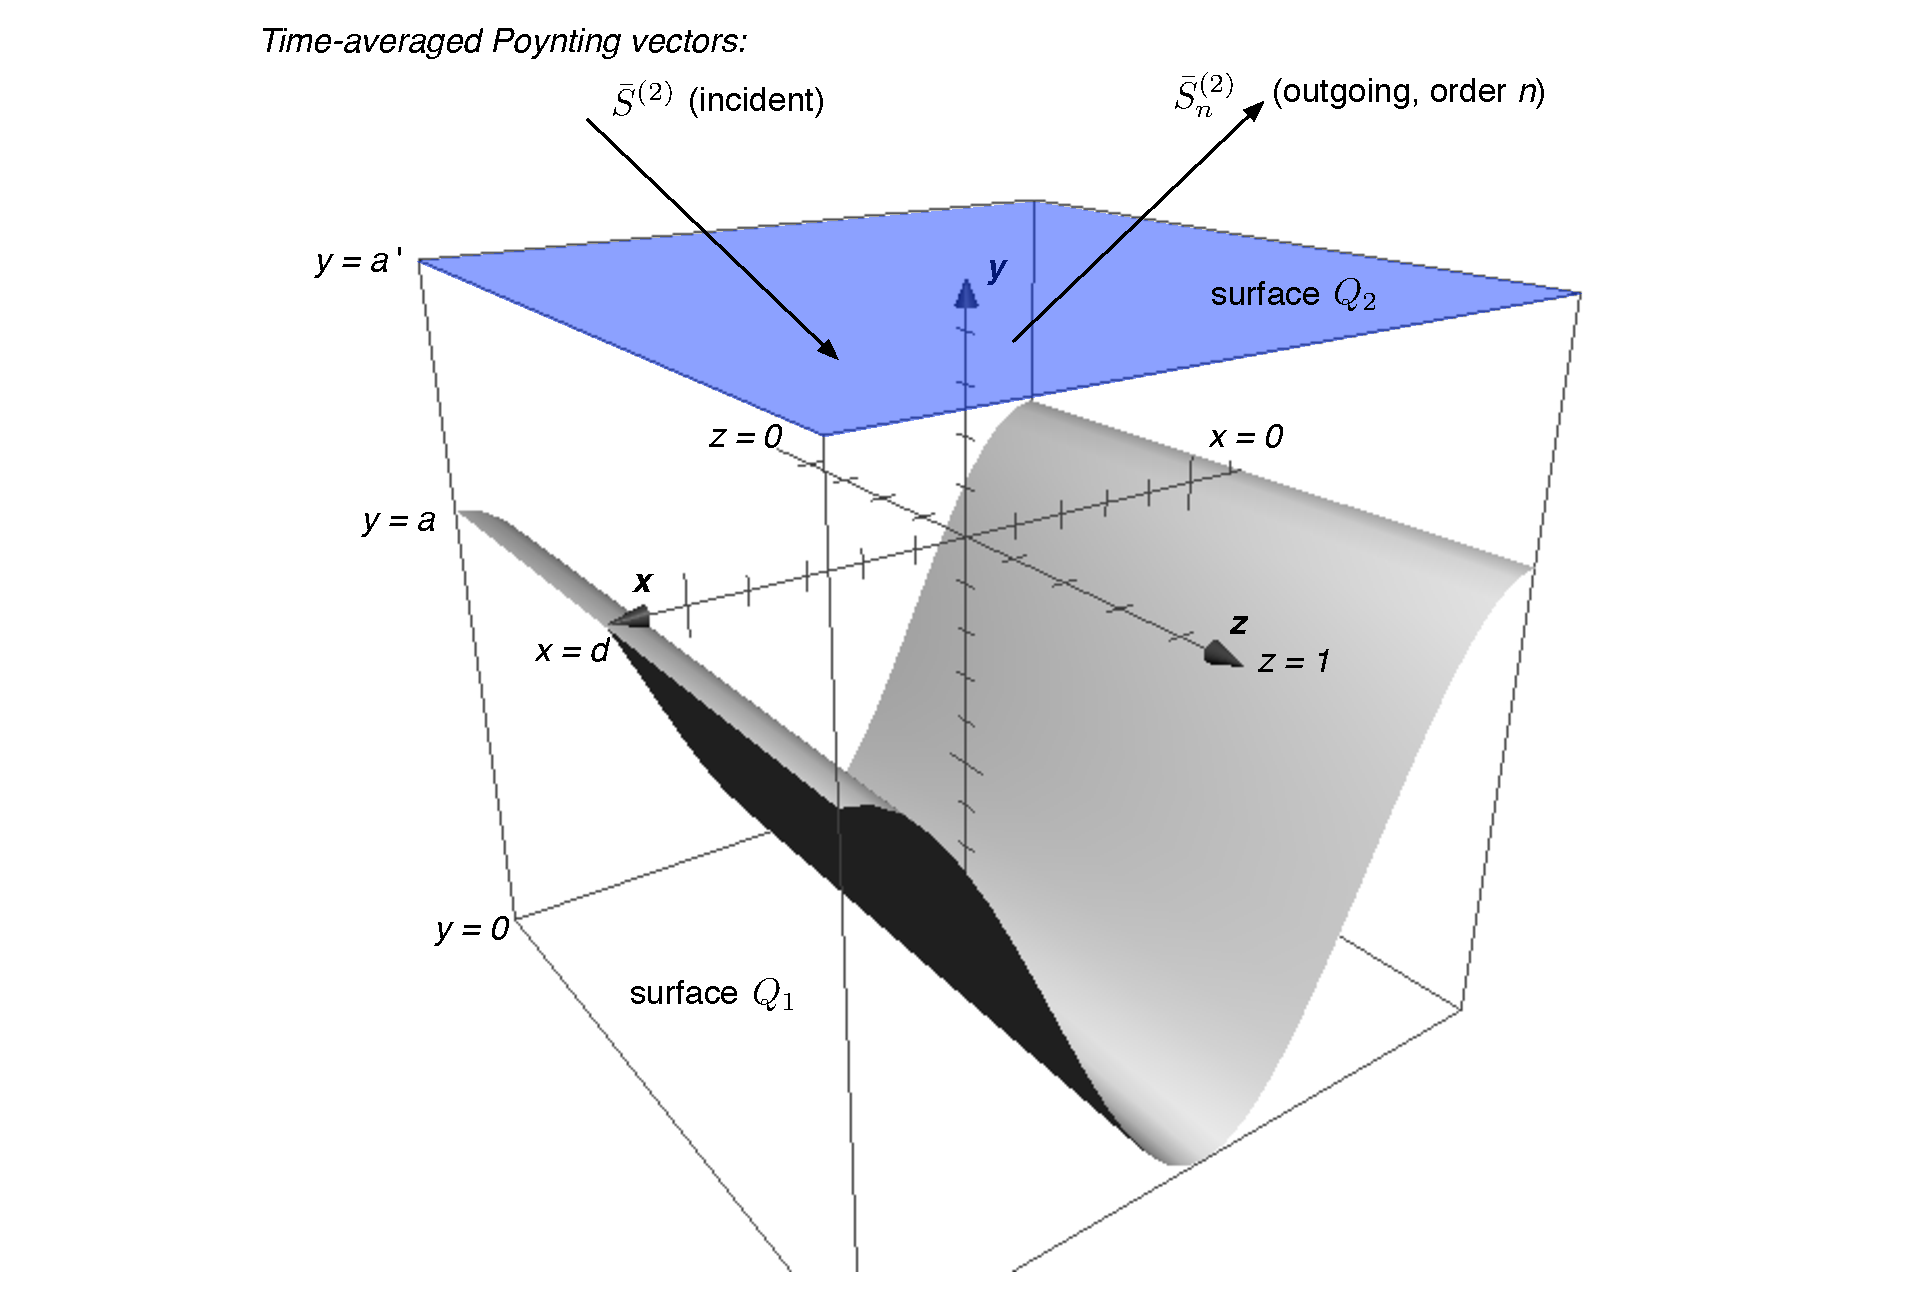
\includegraphics[scale=0.5]{../data/Chapter2/2c_poynting/2c.pdf} 
   \caption{The total electromagnetic flux through this highlighted area ($Q_2$) is used to define the grating efficiency of a diffraction order $n$, as the ratio of the flux of the diffracted wave $\bar S_n^{(2)}$ compared to the incident wave $\bar S^{(2)}$.}
   \label{2c}
\end{figure}

This definition for efficiency can be expressed in terms of the coefficients in the Rayleigh expansion for the reflected and transmitted fields \eq{rayleighExp2}, \eq{rayleighExp1}, so that if we could solve for these coefficients, we would have determined the grating efficiency:
\subsubsection{Reflected Efficiencies}
We know that the incident and diffracted orders are plane waves, so the magnetic field $\vec H$ is related to the electric field $\vec E$ as
\begin{align}
\left| \vec H \right| = \frac{\left| \vec E \right|}{Z_2}
\end{align}
where $Z_2 = v_2 Z_0$ is the impedance of the space above the grating (usually free space, so $v_2=1$ and $Z_2 = Z_0 = 377\Omega$, the impedance of free space). Based on the Rayleigh expansion for the outgoing field (equation \eq{rayleighExp2}), the magnitude of the time-averaged Poynting vector for the \emph{reflected order} is therefore
\begin{align}
\left| \bar S \right| = B_n^{(2)} \, B_n^{(2)\ast} \, \eta_2
\end{align}
where we have defined \fbox{$\eta_2 \equiv 1/(2Z_2)$} in the case of TE polarization, and \fbox{$\eta_2 \equiv 2Z_2$} for TM polarization.  The direction of the vector is along the propagation direction, i.e.: at an angle $\theta_{2,n}$ to the $y$-axis, therefore the integrated flux through the surface is:
\begin{align}
\iint \limits_{Q_2} \bar S_n^{(2)} \, \hat y \, \dif z \dif x &= \int \limits_0^d \int \limits_0^1 \bar S_n^{(2)} \, \hat y \, \dif z \dif x \\
&= B_n^{(2)} \, B_n^{(2)\ast} \, \eta_2 \, d \cos \theta_{2,n} 
\end{align}
For the incident wave, the integrated flux is similarly 
\begin{align}
\iint \limits_{Q_2} \bar S^{(2)} \, \hat y \, \dif z \dif x = A_0^{(2)} \, A_0^{(2)\ast} \, \eta_2 \, d \cos \theta_{2} 
\end{align}
and so the reflected efficiency in order $n$ is:
\begin{align}
e_n^{(r)} &= \frac{    B_n^{(2)} \, B_n^{(2)\ast} \cos \theta_{2,n}       }{    A_0^{(2)} \, A_0^{(2)\ast}  \cos \theta_{2}     }
\end{align}
We can simplify this somewhat by choosing a unit amplitude for the incident field, i.e.: $A_0^{(2)} = 1$V/m for the TE electric field, or 1A/m for the TM magnetic field. Also, since $\beta_n^{(2)} = k_2 \cos \theta_{2,n}$, we can simplify this to
\begin{align}
e_n^{(r)} &= B_n^{(2)} \, B_n^{(2)\ast} \, \frac{     \beta_n^{(2)}       }{    \beta_0^{(2)}      }
\label{eqnEffR}
\end{align}



\subsubsection{Transmitted Efficiencies}
Gratings used in the soft x-ray regime are always used in reflection, due to the high absorption of materials at these wavelengths.  However, since we are working on a general theory with application to all gratings, we can go through the same process for simplifying the transmitted efficiencies.  

Again, we define \fbox{$\eta_1 \equiv 1/(2Z_1)$} in TE polarization, and \fbox{$\eta_1 \equiv 2Z_1)$} in TM polarization, where $Z_1 = v_1 Z_0$ is the impedance of the grating substrate material.  The same integrations over the surface $Q_1$ give the ratio between the total transmitted and incident fluxes:
\begin{align}
e_n^{(t)} &= \frac{    A_n^{(1)} \, A_n^{(1)\ast} \cos \theta_{1,n} \, \eta_1       }{    A_0^{(2)} \, A_0^{(2)\ast}  \cos \theta_{2} \,  \eta_2   }
\end{align}
In this case, the difference in impedance above and below the grooves causes $\eta_1$ and $\eta_2$ to remain in the formula, so the final simplification depends on polarization:
\begin{align}
\label{eqnEffT}
e_n^{(t)} &= A_n^{(1)} \, A_n^{(1)\ast} \frac{  \beta_n^{(1)}   } {  \beta_0^{(2)} }  & \textrm{(TE Polarization)} \\
&= A_n^{(1)} \, A_n^{(1)\ast} \frac{  \beta_n^{(1)}   } {  \beta_0^{(2)} }  \left( \frac{v_2}{v_1} \right)^2 & \textrm{(TM Polarization)}
\end{align}

\section{Solving for efficiency}
To determine $A_n$, $B_n$, and the efficiency, we need to find numerical solutions inside the modulated region for the general wave equations (TE polarization: \eq{wete}, TM polarization: \eq{wetm}). The solutions must match up to the boundary conditions at the top and bottom of the grooves, defined by the Rayleigh expansions \eq{rayleighExp2}, \eq{rayleighExp1}.

The wave equations and electromagnetic boundary conditions now depend on the polarization.  \textbf{In this section, we present the analysis for TE polarization only.}  The approach for TM polarization is similar, but the electromagnetic boundary conditions are different.  The normal component of the TM electric field is discontinuous at the interface; this introduces convergence issues when the Fourier expansions are truncated. A small reformulation is necessary to ensure that the boundary conditions are uniformly satisfied everywhere \cite{Li96b}.  For a detailed application of the differential method in TM polarization, see Reference \cite[Chapter 4]{Nev02}.

\subsection{Representing the grating}

As shown in Figure \ref{2a}, the grating is described by the profile function $y_p = g(x)$, which has a minimum of $y=0$, a maximum $y=a$, and is periodic on $d$:
\begin{align}
y_p = g(x) = g(x+d)
\end{align}
\label{k2Expansion}

\begin{figure}[htbp] %  figure placement: here, top, bottom, or page
   \centering
   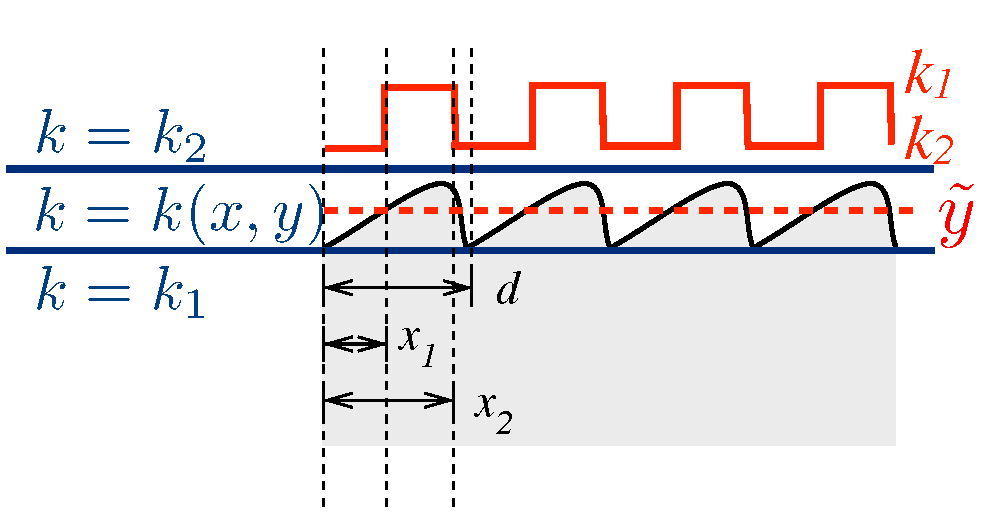
\includegraphics[height=1.6in]{Extended/k2StepFunction.pdf} 
   \caption[The $k^2(x, y)$ function for a simple groove profile.]{The $k^2(x, y)$ function for a simple groove profile. At any height $(0<\tilde y<a)$, the $k^2(x, \tilde y)$ function be a periodic step function going from $k^2_1=(\nu_1 \omega/c)^2$ to $k_2 = (\nu_2 \omega/c)^2$. }
   \label{k2StepFn}
\end{figure}

The exact groove profile is required to determine $k^2$ as a function of position. For a profile of arbitrary shape, at any height $(0<\tilde y<a)$, $k^2(x, \tilde y)$ is a periodic step function going from $k^2_1=(\nu_1 \omega/c)^2$ to $k_2 = (\nu_2 \omega/c)^2$.  We can then determine a Fourier expansion for $k^2$ that applies inside the grooves:  (Note that the expansion is only over $x$; the Fourier coefficients $k^2_n(y)$ are still functions of vertical position $y$.)
\begin{align}
\label{k2FourierExpansion}
k^2(x,\tilde y) = \sum \limits_{n=-\infty}^{\infty} k^2_n(x, \tilde y)\, e^{2\pi i n x/d}
\end{align}
The coefficients $k^2_n$ can be computed using a Fast Fourier Transform of $k^2(x,\tilde y)$ over the period $d$.  Because this is a step function, for simple profiles with discontinuities at $x_1$ and $x_2$ (Figure \ref{k2StepFn}), it can also be computed analytically:
\begin{align}
\sigma_1 &\equiv  k_1^2 - k_2^2 \\
\sigma_2 &\equiv k_2^2 - k_1^2
\end{align}
For $n=0$:
\begin{align}
k^2_0 = \frac{1}{d} \left( k_2^2d - \sigma_1 x_1 - \sigma_2 x_2 \right)
\end{align}
For $n\neq0$:
\begin{align}
k^2_n= \frac{-1}{2 \pi n} \left[ \sigma_1 \left( \sin \left(\frac{2\pi n x_1}{d}\right) + i \cos \left(\frac{2\pi n x_1}{d}\right) \right) +  \sigma_2 \left( \sin \left(\frac{2\pi n x_2}{d}\right) + i \cos \left(\frac{2\pi n x_2}{d}\right) \right) \right]
\end{align}

\subsection{Matrix Formulation of Numerical Solution: Inside the Groooves}
When we put the Fourier expansions for $u_z = E_z$ \eq{eqnFourierExpansionU} and $k^2$ \eq{k2FourierExpansion} into the general differential equation \eq{wete} and truncate to $n=[-N, N]$, we get one second-order differential equation for every $n$:
\begin{align}
\frac{d^2 E_n(y)}{d^2y} + \sum \limits_{m=-N}^{N} k^2_{(n-m)}(y) E_m(y) - \alpha_n^2 E_n(y) = 0
\end{align}
where $E_n$ is the $n^\textrm{th}$ Fourier coefficient in the expansion of the electric field.  This is conveniently expressed by defining the column vector $\left[E(y)\right]$ with $2N+1$ components $E_n(y)$, and the $(2N+1)\times(2N+1)$ square matrix $M$ as
\begin{align}
M_{nm}(y) = -k^2_{(n-m)}(y) + \alpha^2_n \,\delta_{nm}  \qquad \qquad \delta_{nm} = \left\{ \begin{array}{c}1 \textrm{, if } n=m \\0 \textrm{, if } n\neq m\end{array}\right.
\end{align}
%($\delta_{nm}$ is the Kronecker delta, $\delta_{nm} = 1$ for $n=m$, and 0 otherwise.)
giving the matrix equation
\begin{align}
\label{matrixDE}
\frac{d^2 \left[E(y)\right]}{dy^2} = M(y) \, \left[E(y)\right]
\end{align}
This is now a set of second order differential equations in $y$ that need to be solved so that the values of the field coefficients $E_n(y)$ satisfy boundary conditions at the top and bottom of the grooves: $y=a$ and $y=0$.
\subsection{Boundary conditions at the top and bottom of the grooves}
Regardless of the shape of the profile, it always has a maximum value at $y=a$, and a minimum value at $y=0$.  The Maxwell Equations provide two additional boundary conditions here:
\begin{enumerate}
\item The tangential component of the electric field $\vec E$ must be continuous at an interface.

For TE polarization, the tangential component is just the $E_z$ component, so we require that the electric field is continuous at $y=0$ and $y=a$.  Therefore, the field must match up to the Rayleigh expansion solutions found for Region 2 and Region 1:
\begin{align}
\label{boundsA1}
E_n(a) &= A_0^{(2)} e^{-i \beta_0^{(2)} a} \delta_{n,0} + B_n^{(2)} e^{i \beta_n^{(2)}a} \\
\label{bounds01}
E_n(0) &= A_n^{(1)}
\end{align}
At this point, both the $A_n$ and $B_n$ coefficients are still unknown.

\item The tangential component of the magnetic field $\vec H$ must be continuous at an interface.

In TE polarization, the tangential magnetic field is proportional to the normal derivative of the electric field.  At $y=a$ and $y=0$, regardless of the profile shape, the normal vector to the grating surface is along the $y-$direction, so we need $dE_z/dy$ to be continuous; this gives the remaining two boundary conditions:
\begin{align}
\label{boundsA2}
\left. \frac{d E_n(y)}{dy} \right|_{y=a} &= -i \beta_0^{(2)} A_0^{(2)} e^{-i\beta_0^{(2)}a} \delta_{n,0} + i \beta_n^{(2)} B_n^{(2)} e^{i \beta_n^{(2)}a} \\
\label{bounds02}
\left. \frac{d E_n(y)}{dy} \right|_{y=0} &= - i \beta_n^{(1)} A_n^{(1)}
\end{align}

\end{enumerate}

Optionally, these four requirements can be combined to give two equations that link the function $E_n(y)$ to its derivative at $y=0$ and $y=a$:
\begin{align}
\left. \frac{dE_n(y)}{dy} \right|_{y=0} &= - i \beta_n^{(1)} E_n(0)\\
\left. \frac{d E_n(y)}{dy} \right|_{y=a} &=  \left\{   \begin{array}{cl}      i \beta_n^{(2)} E_n(a)   &\qquad (n\neq 0)  \\ -i \beta_0^{(2)} A_0^{(2)} e^{-i\beta_0^{(2)}a}  + i \beta_n^{(2)} \left( E_n(a) - A_0^{(2)} e^{-i \beta_0^{(2)} a} \right)  &\qquad (n=0)  \end{array}   \right.
\end{align}

The four boundary equations (\eq{boundsA1}, \eq{bounds01}, \eq{boundsA2}, \eq{bounds02}), along with the matrix differential equation \eq{matrixDE}, establish the grating boundary value problem (BVP) in the Fourier space, for TE polarization.

\subsection{Solution implementation: The Shooting Method}
\label{shootingMethodDescription}
At this point, we have $2N+1$ second-order boundary value problems that need to be integrated in the $y-$direction \eq{matrixDE}.  In this BVP, the boundary conditions do not provide any values; only a link between the unknown function and its derivative.  To handle this complication, the original theory authors used a technique called the \textbf{{shooting method}} \cite{Pop01}.
% TODO: Other BVP-solving methods are now available, but this method is used by the reference implementation, so we describe it here and use it for the first-generation implementation.

Because the differential equation is a linear system, we can construct a general solution that matches the boundary conditions out of a linear combination of trial solutions.  The Fourier expansion for the field represents a complete basis, so we can use it to generate a complete set of $2N+1$ trial solutions $[\tilde u(y)]_p$ for the vector $[u(y)]$, where $p = [-N, N]$.  Any orthogonal set of particular solutions that satisfies the boundary conditions at $y=0$ \eq{bounds02} is acceptable, so we choose these values for the $p-$th trial solution at $y=0$:
\begin{align}
\label{startingValues}
\tilde E_n(0)_{p} &= \delta_{p,n},\\
\tilde E_n^\prime(0)_{p} &= -i \beta_n^{(1)} \delta_{p,n}.
\end{align}
This transforms the $2N+1$ boundary value problems into $(2N+1)\times(2N+1)$ initial value problems.  All of the trial solutions can now be individually integrated from $y=0$ to $y=a$, using Equation \eq{matrixDE}:
\begin{equation}
[\tilde E^{\prime\prime}(y)]_p = M(y) [\tilde E(y)]_p
\label{matrixDE3}
\end{equation}
using any reliable numerical integration routine.

Finally, we need to find a linear superposition of the trial solutions that satisfies the boundary conditions at $y=a$ \eq{boundsA1}, \eq{boundsA2}:
\begin{align}
\label{superposition1}
\sum \limits_{p=-N}^{+N} c_p \tilde E_{np}(a) &= A_0^{(2)} e^{-i \beta_0^{(2)} a} \delta_{n,0} + B_n^{(2)} e^{i \beta_n^{(2)}a}, \\
\sum \limits_{p=-N}^{+N} c_p \tilde E^\prime_{np}(a) &= -i \beta_0^{(2)} A_0^{(2)} e^{-i\beta_0^{(2)}a} \delta_{n,0} + i \beta_n^{(2)} B_n^{(2)} e^{i \beta_n^{(2)}a}.
\end{align}
Because of the $y=0$ boundary condition \eq{bounds01} and our choice of starting values \eq{startingValues}, the superposition constants $c_p$ can be identified with the coefficients $A^{(1)}_n$: $c_p = A^{(1)}_n$ for $n=p$.  Therefore, these represent $2(2N+1)$ linear equations for the $2(2N+1)$ unknowns $A_n^{(1)}$, $B_n^{(2)}$.  If we eliminate $B_n^{(2)}$, we can express the resulting equations in linear matrix form $A \vec x = \vec b$:
\begin{align}
\label{axb}
T \left[A^{(1)}\right] = \left[V^{(2)}\right],
\end{align}
where $\left[A^{(1)}\right]$ is the vector of $A^{(1)}_n$ coefficients, $\left[V^{(2)}\right]$ is a vector defined by the incident wave (which has a single component when there is only one incident plane wave):
\begin{align}
V^{(2)}_n =  \delta_{n,0} \,e^{-i\beta^{(2)}_0 a},
\end{align}
and $T$ is the square matrix with elements
\begin{align}
T_{np}=   \frac{1}{2} \left[ \tilde E_{np}(a) - \frac{\tilde E^\prime_{np}(a)}{i\beta_n^{(2)}} \right].
\end{align}
Because the grating problem has a unique solution, $T$ must be invertible (as long as the numerical integration process was stable and accurate).  Using $LU$ decomposition or any other standard matrix method to solve the linear system of Equation \eq{axb} provides the coefficients for the transmitted orders $A_n^{(1)}$.  In the final step, Equation \eq{superposition1} provides the $B_n^{(2)}$ coefficients, from which we can compute the reflected efficiencies using Equation \eq{eqnEffR}.

This concludes the basic formulation of the differential method.  However, there are two numerical challenges that complicate its implementation.  One is the truncation convergence issue in TM polarization, which we have already mentioned \cite{Li96b}.  The other is introduced by growing exponential functions that cause a loss of significance during the numerical integration.

\subsection{Integration of growing exponentials: The S-Matrix method}
\label{SMatrixMethod}
The integration process \eq{matrixDE3} requires numerically integrating a set of growing and decaying exponential functions.  As the groove depth, or integration distance $a$ increases, the values of $\tilde u_p$ and $\tilde u'_p$ become very large -- for example, on the order of $10^{22}$ for a depth of just $a = 0.1$ um.  However, the algebraic process \eq{axb} requires taking the sum and difference of many large $\tilde u_p$ values to produce a number less than unity.  On a computer with finite-precision floating point numbers, this results in a loss of significance that can make the final result meaningless.

For example, standard double-precision (IEEE 754) variables have a decimal precision of approximately 16 digits.  The subtraction of two numbers on the order of $10^{22}$ will have a result precision of $\pm10^6$.  Obviously, a final efficiency result of $e_{r,1} = 0.21 \pm 10^6$ would be of little use.  To mitigate this, we need a strategy to keep the $\tilde u_p$ values bounded within the significant range; the only way to accomplish this is to limit the integration distance.

The solution to this problem was originally developed for handling stacks of grating layers, like those shown in Figure \ref{2d-1}.  Here, the grating is sliced into layers between modulated regions (Figure \ref{2d-2}).  However, the technique can also be applied to a single deep grating, as shown in Figure \ref{2d-3}, where the layer thicknesses are chosen small enough to keep the integration values bounded.  The basic concept is to conduct separate numerical integrations using assumed starting values from the bottom to the top of each layer, and then to combine the effects of all layers using a stable matrix algorithm.

\begin{figure}[htbp] %  figure placement: here, top, bottom, or page
   \centering
   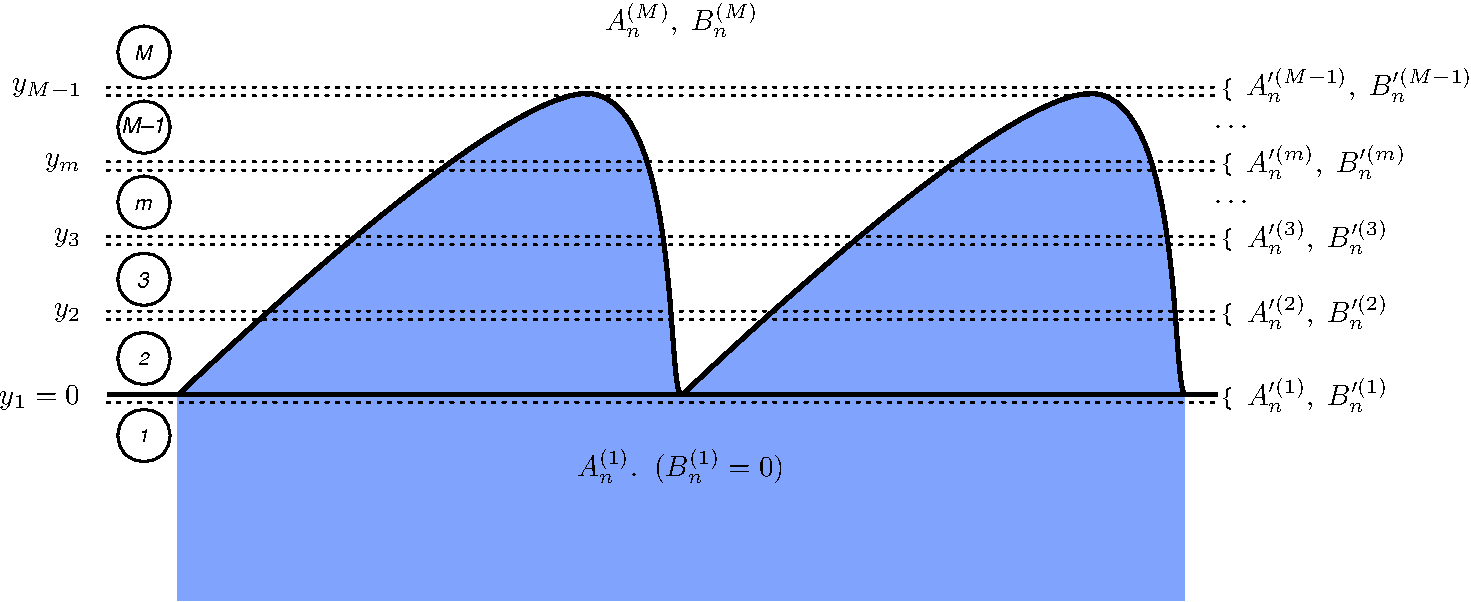
\includegraphics[width=\textwidth]{Chapter2/2d_stacksOfGratings/2d_3.pdf} 
   \caption[Using the S-matrix method, thick gratings are divided into layers, where each layer is thin enough to avoid losing numerical significance during integration.]{Using the S-matrix method, thick gratings are divided into layers, where each layer is thin enough to avoid losing numerical significance during integration.  Conceptually, we insert a zero-thickness homogeneous layer between each ``real'' region, so that Rayleigh expansions with coefficients $A'_n,\, B'_n$ are valid.  (These conceptual layers have the same impedance $(k_M^2)$ and $\beta_n^{(M)}$ as the vacuum region $M$.)}
   \label{2d-3}
\end{figure}

Between each ``real'' grating layer (Figure \ref{2d-3}), we can conceptually insert a homogeneous layer with zero thickness.  By giving the conceptual layer the same refractive index as the vacuum, we ensure that the Rayleigh expansion that applies within it has the same $\beta_n$ values and propagation angles as the Rayleigh expansion above the grating.  (Introducing this conceptual layer has no effect on the grating efficiency, because it has zero thickness; we introduce it only to make the mathematics convenient.)

Previously, in the single-layer formulation, we had a single down-going wave $A^{(2)}_0$ above the grating, and a set of up-going reflected waves $B^{(2)}_n$.  Below the grating (inside the substrate) there was a set of down-going transmitted waves $A^{(1)}_n$.  In the multi-layer formulation, we now have down-going and up-going waves within each conceptual layer.  Instead of just one incident wave, all except the external layers have a complete set of waves incident from both above and below.  Transmitted light from the region above creates down-going incident waves; reflected light from the region below creates up-going incident waves.

Figure \ref{2d-3} shows the numbering we adopt now for the conceptual homogeneous layers.  They are numbered from $m=1$ (the substrate) to $m=M-1$.  The number of ``real'' grating slices is $M-2$, and the vacuum region above the grating is labelled  $M$.  Within each conceptual layer $m$, at a height $y_m$, the field is described by a Rayleigh expansion with coefficients $A'^{(m)}_n$ and $B'^{(m)}_n$:
\begin{align}
E_z(x,y) &= \sum\limits_{n=-N}^{N} \left[ A'^{(m)}_n  e^{-i \beta^{(M)}_n y_m}   +  B'^{(m)}_n e^{i \beta^{(M)}_n y_m} \right] e^{i \alpha_n x}.
\label{rayleighS}
\end{align}
Because we have chosen the conceptual layers to have the same refractive index as the vacuum, $\beta^{(m)}_n = \beta^{(M)}_n$.  Since the top conceptual layer is in the vacuum above the grating, $A'^{(M-1)}_n = A^{(M)}_n$ and $B'^{(M-1)}_n = B^{(M)}_n$.

To simplify the matrix calculations, we define a vector $V^{(m)}$ with two blocks to represent the up-going and down-going waves inside each conceptual layer.  Each block contains the components for all orders $n$:
\begin{equation}
V^{(m)} \equiv  \left(\begin{array}{c}\vdots \\ A'^{(m)}_n  e^{-i \beta^{(M)}_n y_m} \\ \vdots \\\hline \vdots \\ B'^{(m)}_n e^{i \beta^{(M)}_n y_m} \\ \vdots\end{array}\right) 
\end{equation}
We can then define a (yet unknown) \textbf{transmission matrix} $T^{(m)}$ for the $m$-th conceptual layer that describes the effect of the region directly below it:
\begin{align}
V^{(m)} = T^{(m)} V^{(m-1)}
\end{align}
This relates the waves in the $(m-1)^\textrm{th}$ conceptual layer to the $m^\textrm{th}$ conceptual layer.

If we could compute the $T^{(m)}$ matrix for each layer, the transmission matrix for the total stack $T$ could be found, relating the waves at the top of the stack ($m=M$) to the waves at the bottom ($m=1,\, y=0$):
\begin{align}
\left(\begin{array}{c}\vdots \\ A^{(M)}_n  e^{-i \beta^{(M)}_n y_m} \\ \vdots \\\hline \vdots \\ B^{(M)}_n e^{i \beta^{(M)}_n y_m} \\ \vdots\end{array}\right)  &= T \left(\begin{array}{c}\vdots \\ A^{(1)}_n \\ \vdots \\\hline \vdots \\ B^{(1)}_n \\ \vdots\end{array}\right),
\end{align}
where
\begin{align}
T &= T^{(M-1)} \ldots T^{(m)} \ldots T^{(3)} T^{(2)}.
\end{align}

There are no up-going waves incident from below the substrate, so $B^{(1)}_n = 0$:
\begin{align}
\left(\begin{array}{c}\vdots \\ A^{(M)}_n  e^{-i \beta^{(M)}_n y_m} \\ \vdots \\\hline \vdots \\ B^{(M)}_n e^{i \beta^{(M)}_n y_m} \\ \vdots\end{array}\right)  &= T \left(\begin{array}{c}\vdots \\ A^{(1)}_n \\ \vdots \\\hline \vdots \\ 0 \\ \vdots\end{array}\right)
\label{tMatrixFullStack}
\end{align}
This equation is sufficient to calculate the outgoing transmitted waves $A^{(1)}_n$ and reflected waves $B^{(M)}_n$ for any incidence condition $A_n^{(M)}$.

\subsubsection{Determining the T-matrix for one layer}
To determine the $T^{(m)}$ matrix that describes the region below the $m^\textrm{th}$ conceptual layer, we again apply the shooting method.  Like in Section \ref{shootingMethodDescription}, we generate a set of $P$ orthogonal trial solution vectors $V^{(m-1)}_p$ that satisfy the boundary conditions at the bottom of the region, and integrate them numerically from $y_{m-1}$ to $y_{m}$.  Then, we choose a linear combination of the resulting $V^{(m)}_p$ that satisfy the boundary conditions at the top ($y_m$).  However, because we now have up-going \emph{and} down-going incident waves within the region, we need twice as many trial solutions as before: $P=2(2N+1)$.

As a reminder, the boundary conditions now require that our numerical solution within the modulated region below $y_m$ must match up to the Rayleigh expansions defined in the conceptual layers above and below. The boundary conditions come from the continuity of the tangential electric field $\left(E_z = \sum E_n(y) \exp{\left(i \alpha_n x\right)} \right)$ and its first derivative at $y_{m-1}$ and $y_m$:
\begin{align}
\label{eqnBounds1S}
E_n(y_{m-1}) &= A'^{(m)}_n e^{-i \beta^{(M)}_n y_{m-1}} + B'^{(m)} e^{i \beta^{(M)}_n y_{m-1}} \\
\label{eqnBounds2S}
\left. \frac{dE_n}{dy} \right|_{y_{m-1}} &= -i \beta^{(M)}_n A'^{(m)}_n e^{-i \beta^{(M)}_n y_{m-1}} + i \beta^{(M)}_n B'^{(m)}_n e^{i \beta^{(M)}_n y_{m-1}}  \\
\label{eqnBounds3S}
E_n(y_m) &= A'^{(m)}_n e^{-i \beta^{(M)}_n y_m} + B'^{(m)} e^{i \beta^{(M)}_n y_m} \\
\label{eqnBounds4S}
\left. \frac{dE_n}{dy} \right|_{y_m} &= -i \beta^{(M)}_n A'^{(m)}_n e^{-i \beta^{(M)}_n y_m} + i \beta^{(M)}_n B'^{(m)}_n e^{i \beta^{(M)}_n y_m}
\end{align}


Therefore, we choose the following trial solutions at $y_{m-1}$.  For the first $2N+1$ solutions (from $p=[-N,N]$), we use a vector 
\begin{align}
V^{(m-1)}_{p} &=   \left(\begin{array}{c}\vdots \\   A'^{(m-1)}_n  e^{-i \beta^{(M)}_n y_{m-1}}  \\ \vdots \\\hline \vdots \\  B'^{(m-1)}_n  e^{i \beta^{(M)}_n y_{m-1}}  \\ \vdots \end{array}\right)  =  \left(\begin{array}{c} \vdots \\  \delta_{n,p}  \\ \vdots \\\hline \vdots \\ 0 \\ \vdots \end{array}\right),
\end{align}
and derivatives
\begin{align}
\frac{V^{(m-1)}_{p}}{dy} &=  \left(\begin{array}{c} \vdots \\  -i \beta^{(M)}_n \delta_{n,p}   \\ \vdots  \\\hline \vdots \\ 0 \\ \vdots \end{array}\right).
\end{align}
From \eq{rayleighS}, these correspond to starting integration values for the trial electric field components $\tilde E_{n,p}$ at $y_{m-1}$:
\begin{align}
\tilde E_{n,p} (y_{m-1}) &= A'^{(m-1)}_n e^{-i \beta^{(m-1)}_n y_{m-1}} + B'^{(m-1)}_n e^{i \beta^{(m-1)}_n y_{m-1}} = \delta_{n,p} + 0 ,\\
\left. \frac{d \tilde E_{n,p}}{dy} \right|_{y_{m-1}} &= -i \beta^{(M)}_n \delta_{n,p}.
\end{align}


For the second set of $2N+1$ trial solutions (from $p=[N+1,3N+1]$) we choose down-going waves for starting values:
\begin{align}
V^{(m-1)}_{p} &=   \left(\begin{array}{c}\vdots \\   A'^{(m-1)}_n  e^{-i \beta^{(M)}_n y_{m-1}}  \\ \vdots \\\hline \vdots \\  B'^{(m-1)}_n  e^{i \beta^{(M)}_n y_{m-1}}  \\ \vdots \end{array}\right)  =  \left(\begin{array}{c} \vdots \\   0   \\ \vdots  \\\hline \vdots \\  \delta_{n,p-(2N+1)}  \\ \vdots \end{array}\right),
\end{align}
with derivatives
\begin{align}
\frac{V^{(m-1)}_{p}}{dy} &=  \left(\begin{array}{c} \vdots \\  0   \\ \vdots \\\hline \vdots \\   i \beta^{(M)}_n \delta_{n,p-(2N+1)}   \\ \vdots \end{array}\right).
\end{align}
These correspond to starting values of the electric field components
\begin{align}
\tilde E_{n,p} (y_{m-1}) &= A'^{(m-1)}_n e^{-i \beta^{(m-1)}_n y_{m-1}} + B'^{(m-1)}_n e^{i \beta^{(m-1)}_n y_{m-1}} = 0 + \delta_{n,p-(2N+1)}, \\
\left. \frac{d \tilde E_{n,p}}{dy} \right|_{y_{m-1}} &= i \beta^{(M)}_n \delta_{n,p-(2N+1)}.
\end{align}

Now we can numerically integrate the electric field components from $y_{m-1}$ to $y_m$ as before, using Equation \eq{matrixDE}.  From the second pair of boundary conditions \eq{eqnBounds3S}\eq{eqnBounds4S}, we can compute $V^{(m)}_p$ at the end of the integration:
\begin{align}
V^{(m)}_{p} &=   \left(\begin{array}{c}\vdots \\   A'^{(m)}_n  e^{-i \beta^{(M)}_n y_{m}}  \\ \vdots \\\hline \vdots \\  B'^{(m)}_n  e^{i \beta^{(M)}_n y_{m}}  \\ \vdots \end{array}\right)  =  \left(\begin{array}{c} \vdots \\        \frac{1}{2}\left( \tilde E_{n,p}(y_m) - \frac{1}{i\beta^{(M)}_n}\frac{d\tilde E_{n,p}}{dy}(y_m)   \right)            \\ \vdots  \\\hline \vdots \\            \frac{1}{2}\left( \tilde E_{n,p}(y_m) + \frac{1}{i\beta^{(M)}_n}\frac{d\tilde E_{n,p}}{dy}(y_m)   \right)             \\ \vdots \end{array}\right).
\end{align}
Because of the fortunate choice of starting values $V^{(m-1)}_{n,p} = \delta_{n,p}$, 
the solution to the matrix equation
\begin{align}
V^{(m)} = T^{(m)} V^{(m-1)}
\end{align}
is easy and direct:
\begin{align}
T^{(m)}_{n,p} = V^{(m)}_{n,p}.
\end{align}
The shooting method, when used with this choice of starting values, directly determines the components of the $m$-th layer's $T^{(m)}$ matrix.

\subsubsection{The combined efficiency of a stack of layers}
Mathematically, having determined the $T^{(m)}$ matrix for each layer, we can compute the combined effect of the whole stack through matrix products
\begin{align}
T &= T^{(M-1)} \ldots T^{(m)} \ldots T^{(3)} T^{(2)},
\end{align}
and use Equation \eq{tMatrixFullStack} to determine the final transmitted waves $A^{(1)}_n$ and reflected waves  $B^{(M)}_n$ for any incidence condition $A_n^{(M)}$.  Numerically, however, this matrix multiplication results in the exact same large numbers and loss of significance that we originally set out to avoid.

We recall that the layers were chosen sufficiently thin to keep the $T^{(m)}$ matrix for each layer bounded within significance; the problem enters in the multiplication.  Fortunately, we can use an algebraic re-formulation to avoid ever having to compute the full matrix product $T$.  The \textbf{S-matrix propagation algorithm} was discovered by Li \cite{Li96} and applied to the differential method by Neviere and Montiel \cite{Nev96}.  Instead a matrix $T^{(m)}$ that describes the effect of one layer, it defines the matrix $S^{(q)}$ that describes the cumulative effect of \emph{all layers from $m=1$ up to the $q^\textrm{th}$ layer}:
%\begin{equation}
% \left(\begin{array}{c}\vdots \\ B'^{(q)}_n  e^{i \beta^{(M)}_n y_q} \\ \vdots \\\hline \vdots \\ A^{(1)}_n e^{-i \beta^{(M)}_n y_1} \\ \vdots\end{array}\right) = S^{(q)} \left(\begin{array}{c}\vdots \\ B^{(1)}_n  e^{i \beta^{(M)}_n y_1} \\ \vdots \\\hline \vdots \\ A'^{(q)}_n e^{-i \beta^{(M)}_n y_q} \\ \vdots\end{array}\right) 
%\end{equation}
\begin{equation}
 \left(\begin{array}{c}\vdots \\ B'^{(q)}_n  e^{i \beta^{(M)}_n y_q} \\ \vdots \\\hline \vdots \\ A^{(1)}_n \\ \vdots\end{array}\right) = S^{(q)} \left(\begin{array}{c}\vdots \\ B^{(1)}_n  \\ \vdots \\\hline \vdots \\ A'^{(q)}_n e^{-i \beta^{(M)}_n y_q} \\ \vdots\end{array}\right) 
 \label{sMatrixDef}
\end{equation}
The $S$ matrix is bounded by definition, and its blocks have well-defined physical interpretations as reflection and transmission matrices \cite[Chapter 3]{Nev02}.  The algorithm re-arranges the blocks of the T-matrices so that the growing exponential functions never appear in the result.

The S-matrix algorithm is derived in inductive fashion by writing out \eq{sMatrixDef} at levels $q$ and $q+1$.  We omit the algebra here and state only the final results.  To start, we split the $T$ and $S$ matrices into square blocks of size $2N+1$:
\begin{align}
T &= \left[\begin{array}{c|c}T_{11} & T_{12} \\\hline T_{21} & T_{22}\end{array}\right] \\
S &= \left[\begin{array}{c|c}S_{11} & S_{12} \\\hline S_{21} & S_{22}\end{array}\right]
\end{align}
Defining a temporary matrix $Z^{(q)}$:
\begin{align}
\label{SmatZ}
Z^{(q)} &\equiv \left(T^{(q+1)}_{11} + T^{(q+1)}_{12}S^{(q)}_{12} \right)^{-1},
\end{align}
the results allow us to express the $S$ matrix up to the $q+1$ layer based on the $S$ matrix at the $q^\textrm{th}$ layer and the T-matrix of the $(q+1)^\textrm{th}$ layer:
\begin{align}
\label{Smat22}
S^{(q+1)}_{22} &= S^{(q)}_{22} Z^{(q)} \\
\label{Smat12}
S^{(q+1)}_{12} &= \left(T^{(q+1)}_{21} + T^{(q+1)}_{22}S^{(q)}_{12} \right) Z^{(q)}
\end{align}
(The other two blocks of the $S$ matrix can also be calculated, but are not actually required to determine the efficiencies, or proceed with the algorithm.)
\begin{align}
S^{(q+1)}_{21} &= S^{(q)}_{21} - S^{(q+1)}_{22} T^{(q+1)}_{12} S^{(q)}_{11} \\
S^{(q+1)}_{11} &= - S^{(q+1)}_{12} T^{(q+1)}_{12} S^{(q)}_{11} + T^{(q+1)}_{22}S^{(q)}_{11}
\end{align}
Equation \eq{SmatZ}, \eq{Smat22}, and \eq{Smat12} give us exactly what we need to iterate vertically through a stack of grating layers.  The calculation of the $S$ matrix for a full grating begins at layer 1, where no reflection occurs and the transmission is unity for all incoming waves:
\begin{align}
S^{(1)}_{12} &= 0\\
S^{(1)}_{22} &= \mathbb{1}
\end{align}
Applying the inductive step at the top of the first layer ($y=y_2$) gives:
\begin{align}
Z^{(1)} &= \left(T^{(2)}_{11}  \right)^{-1} \\
S^{(2)}_{12} &= T^{(2)}_{21}  \left(T^{(2)}_{11}  \right)^{-1} \\
S^{(2)}_{22} &= \left(T^{(2)}_{11}  \right)^{-1}
\end{align}
The rest of the stack is solved inductively by computing the $T^{(q+1)}$ matrix at each layer $q+1$, and then using Equation \eq{SmatZ}, \eq{Smat22}, and \eq{Smat12} to determine $S^{(q+1)}$, until we reach the top layer.

Finally, we can use the blocks of the final $S^{(M-1)}$ matrix to relate the incident waves at the top of the grating to the diffracted and transmitted waves, using Equation \eq{sMatrixDef}. Since there are no up-going waves incident from below the substrate $(B_n^{(1)} = 0)$:
\begin{equation}
 \left(\begin{array}{c}\vdots \\ B^{(M)}_n  e^{i \beta^{(M)}_n y_{M-1}} \\ \vdots \\\hline \vdots \\ A^{(1)}_n \\ \vdots\end{array}\right) =            \left[\begin{array}{c|c}S^{(M-1)}_{11} & S^{(M-1)}_{12} \\\hline S^{(M-1)}_{21} & S^{(M-1)}_{22}\end{array}\right]       \left(\begin{array}{c}\vdots \\ 0  \\ \vdots \\\hline \vdots \\ A^{(M)}_n e^{-i \beta^{(M)}_n y_{M-1}} \\ \vdots\end{array}\right) 
 \label{sMatrixDef}
\end{equation}
For a single incident plane wave with normalized intensity, $A_n^{(M)} = \delta_{n,0}$.  From this we can work out the transmitted Rayleigh coefficients below the grating
\begin{align}
A_n^{(1)} &= S_{22,n,0}^{(M-1)} e^{-i \beta_0^{(M)}y_{M-1}},
\end{align}
and the diffracted Rayleigh coefficients above the grating
\begin{align}
B_n^{(M)} &= S_{12,n,0}^{(M-1)} e^{-i (\beta_n^{(M)} + \beta_0^{(M)}) y_{M-1}}.
\end{align}
Having computed the outgoing Rayleigh coefficients without loss of significance, Equations \eq{eqnEffR} and \eq{eqnEffT} compute the final reflected and transmitted efficiencies in each diffraction order.

\section{Interaction of X-rays and materials}
In setting up the differential theory, we assumed that light propagation within the grating material could be described by a refractive index, but we failed to suggest what this refractive index would be, and how it would vary with wavelength.  In this final theory section, we verify the assumption and suggest one source of refractive index data.

In the soft x-ray region, the refractive index description is generally valid -- both for conventional dielectrics like SiO$_2$, and for metals.  In metals, the frequency of x-ray light is much higher than the plasma frequency; free electrons cannot respond fast enough to follow the changing electric field, so the material behaves as a weak dielectric rather than a conductor.  However, the incident x-rays are sufficiently energetic to cause electronic state transitions in bound electrons (\textbf{photoabsorption}); the result is substantial attenuation of the beam as it propagates through the material.  Energy in the beam is also lost through \textbf{coherent scattering} of photons off electrons in the material.  These two processes mean that attenuation is always present, but it becomes extremely strong at photon energies immediately above the material's \textbf{absorption edges}.

The complex refractive index $\nu$
\begin{align}
\nu(\lambda) = n + i \kappa
\end{align}
can describe both the dielectric strength and the attenuation.  The real component $n$ is analogous to the conventional refractive index; it describes the phase velocity $v$ of the light in the material,
\begin{align}
n = c / v,
\end{align}
while the \textbf{extinction coefficient }$\kappa$ describes the amount of attenuation.  When using the sign convention for the electric field in Equation \eq{eqnPlaneWave},
\begin{align}
E \propto \exp(i(kz - \omega t)) = \exp(i \omega(\nu z/c - t)),
\end{align}
the sign of $\kappa$ must be positive for absorption.  ($\kappa < 0$ would imply amplification as the light travelled through the material.)
For almost all materials at x-ray wavelengths, $n$ is smaller than, but very close to one, so the refractive index is often listed as
\begin{align}
\nu = 1 - \delta + i \kappa
\end{align}

\subsection{Atomic scattering factors and the refractive index}
\label{secHenke}
At soft x-ray wavelengths, it nearly impossible to measure the refractive index directly.  Instead, scattering theory and absorption measurements can be used together to determine semi-empirical values.  Scattering of electromagnetic waves from single point charges (e.g., electrons) is well described by classical \textbf{Thomson scattering}.  To extend this to multi-electron situations, the \textbf{atomic scattering factor} $f$ describes the amplitude of an electromagnetic wave scattered by a complete atom, compared to what would be scattered by a single electron.
\begin{align}
f = f_1 + i f_2
\end{align}
It is complex because all of the atom's electrons might not scatter in phase.  It can be separated into a forward-scattering component $f(0)$ and a correction $\Delta f_0$ that depends on the scattering angle $\theta$:
\begin{align}
f = f_1 + i f_2 = f_1(0) - \Delta f_0(\theta) + i f_2(0)
\end{align}
The ``Henke Data'' publication \cite{Hen93} tabulates the atomic scattering factors for all elements from Hydrogen to Uranium over the energy range from 50 eV to 30~000 eV.  The authors calculate the scattering factors from a survey of all existing available photoabsorption measurements.  The measured absorption cross section directly provides the imaginary part of the scattering factor ($f_2$).  Since it is practically impossible to empirically measure the speed of x-ray light in absorbing materials, the Kramers-Kronig dispersion relations are used to determine the real part ($f_1$) from the imaginary part \cite{Kro26}.  (A modified Kramers-Kronig dispersion relation is used to correct for relativistic effects.)  Across energy regions where photoabsorption measurements were not available, the values were interpolated using theoretical calculations.

If the atoms within a material (metal, molecule, or crystal) can be assumed to scatter as dipoles, the complex refractive index can be determined from the scattering factors of all the constituent atoms. This allows us to estimate the refractive index -- even for compound grating materials like SiO$_2$ and MgF$_2$ -- as a function of wavelength:
\begin{align}
\tilde n = 1 - \delta - i \beta = 1 - \frac{r_e}{2\pi} \lambda ^2 \sum\limits_{q=1}^Q n_q f_q(0),
\label{nFromScatteringFactor}
\end{align}
where there are $Q$ different types of atoms in the material, $n_q$ is the number density of atoms of type $q$, $f_q(0)$ is the complex forward scattering factor $f(0)$ for atom $q$, and $r_e$ is the classical electron radius \cite{Hen93}.    (Note that the refractive index $\tilde n$ here uses the opposite sign convention to $\nu$ defined above; if $\tilde n = 1 - \delta - i \beta$,  $\nu = 1 - \delta + i \beta$.)

Using this method to calculate the refractive index assumes that the photoabsorption cross section does not depend on the bonding environment of atoms in the material; i.e., \emph{it assumes that the individual atoms scatter independently}.  In the vicinity of absorption edges, two processes invalidate this assumption: transitions to weakly bound excited states produce fine structure near the absorption edge (NEXAFS), and backscattering of outgoing photoelectrons from the atoms in a crystal causes oscillations above the edge (EXAFS).

Given these effects, is it acceptable to use refractive indexes derived from the Henke data?  Two examples from Reference \cite{Hen93} show the limits of validity.  Figure \ref{henkeValid1} compares the reflectivity of a pure silicon wafer calculated from atomic scattering factors against measurements of the real crystal; in this case the agreement is good.  In Figure \ref{henkeValid2}, the near-edge absorption fine structure of CO$_2$ causes deviation in the measured absorption spectrum compared to the vector sum of the atomic photoabsorption in the vicinity of the Carbon K 1s and Oxygen K 1s absorption edges.

\begin{figure}[htbp] %  figure placement: here, top, bottom, or page
   \centering
   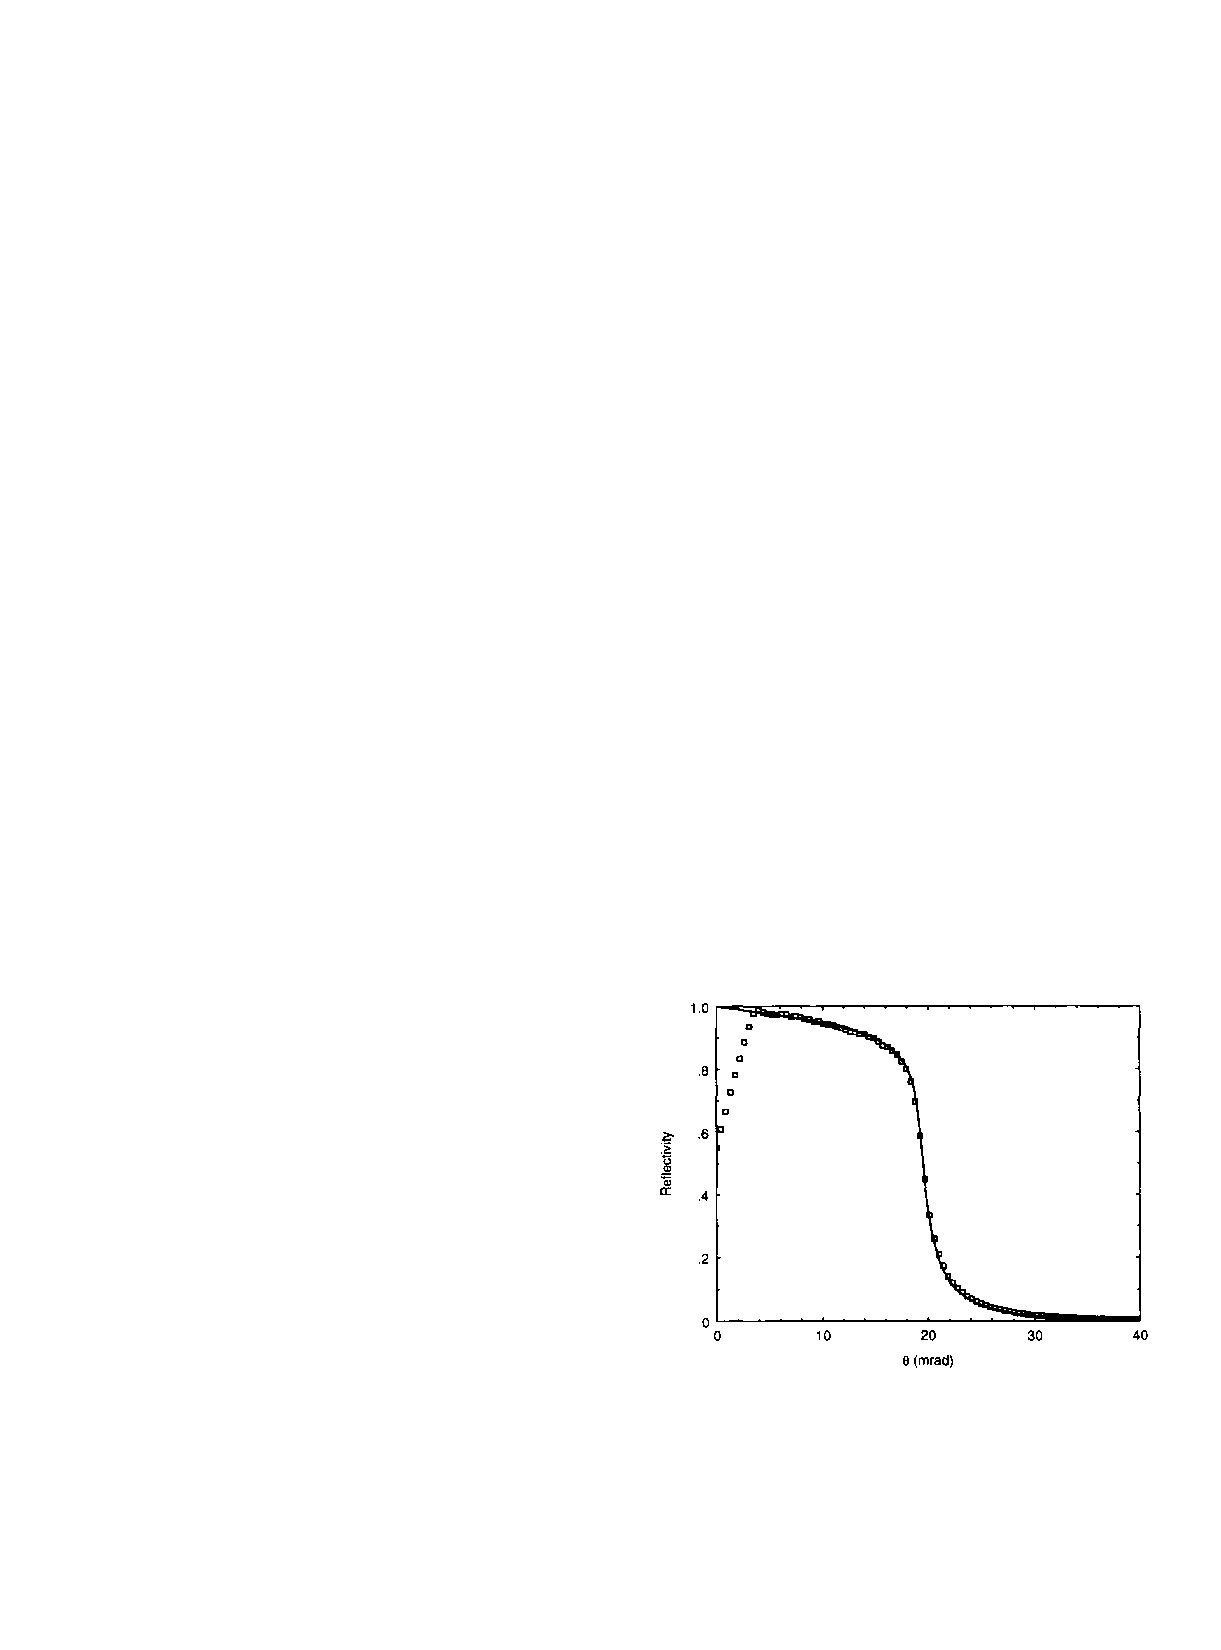
\includegraphics[width=4in]{Chapter2/2f_henke/siReflectivity.pdf} 
   \caption[Comparison of a measured reflection curve around the total reflection cutoff region from a silicon(111) wafer under 1487 eV radiation, with that predicted by the Fresnel equations using atomic scattering factors from the Henke tables.]{Comparison of a measured reflection curve around the total reflection cutoff region from a silicon(111) wafer under 1487 eV radiation, with that predicted by the Fresnel equations (\protect \eq{eqnFresnelTE}, \protect \eq{eqnFresnelTM}) using the atomic scattering factors from the Henke tables. (The low-angle cutoff is instrumental.) Reprinted from Reference \protect \cite[Figure 18]{Hen93}.}
   \label{henkeValid1}
\end{figure}
\begin{figure}[htbp] %  figure placement: here, top, bottom, or page
   \centering
   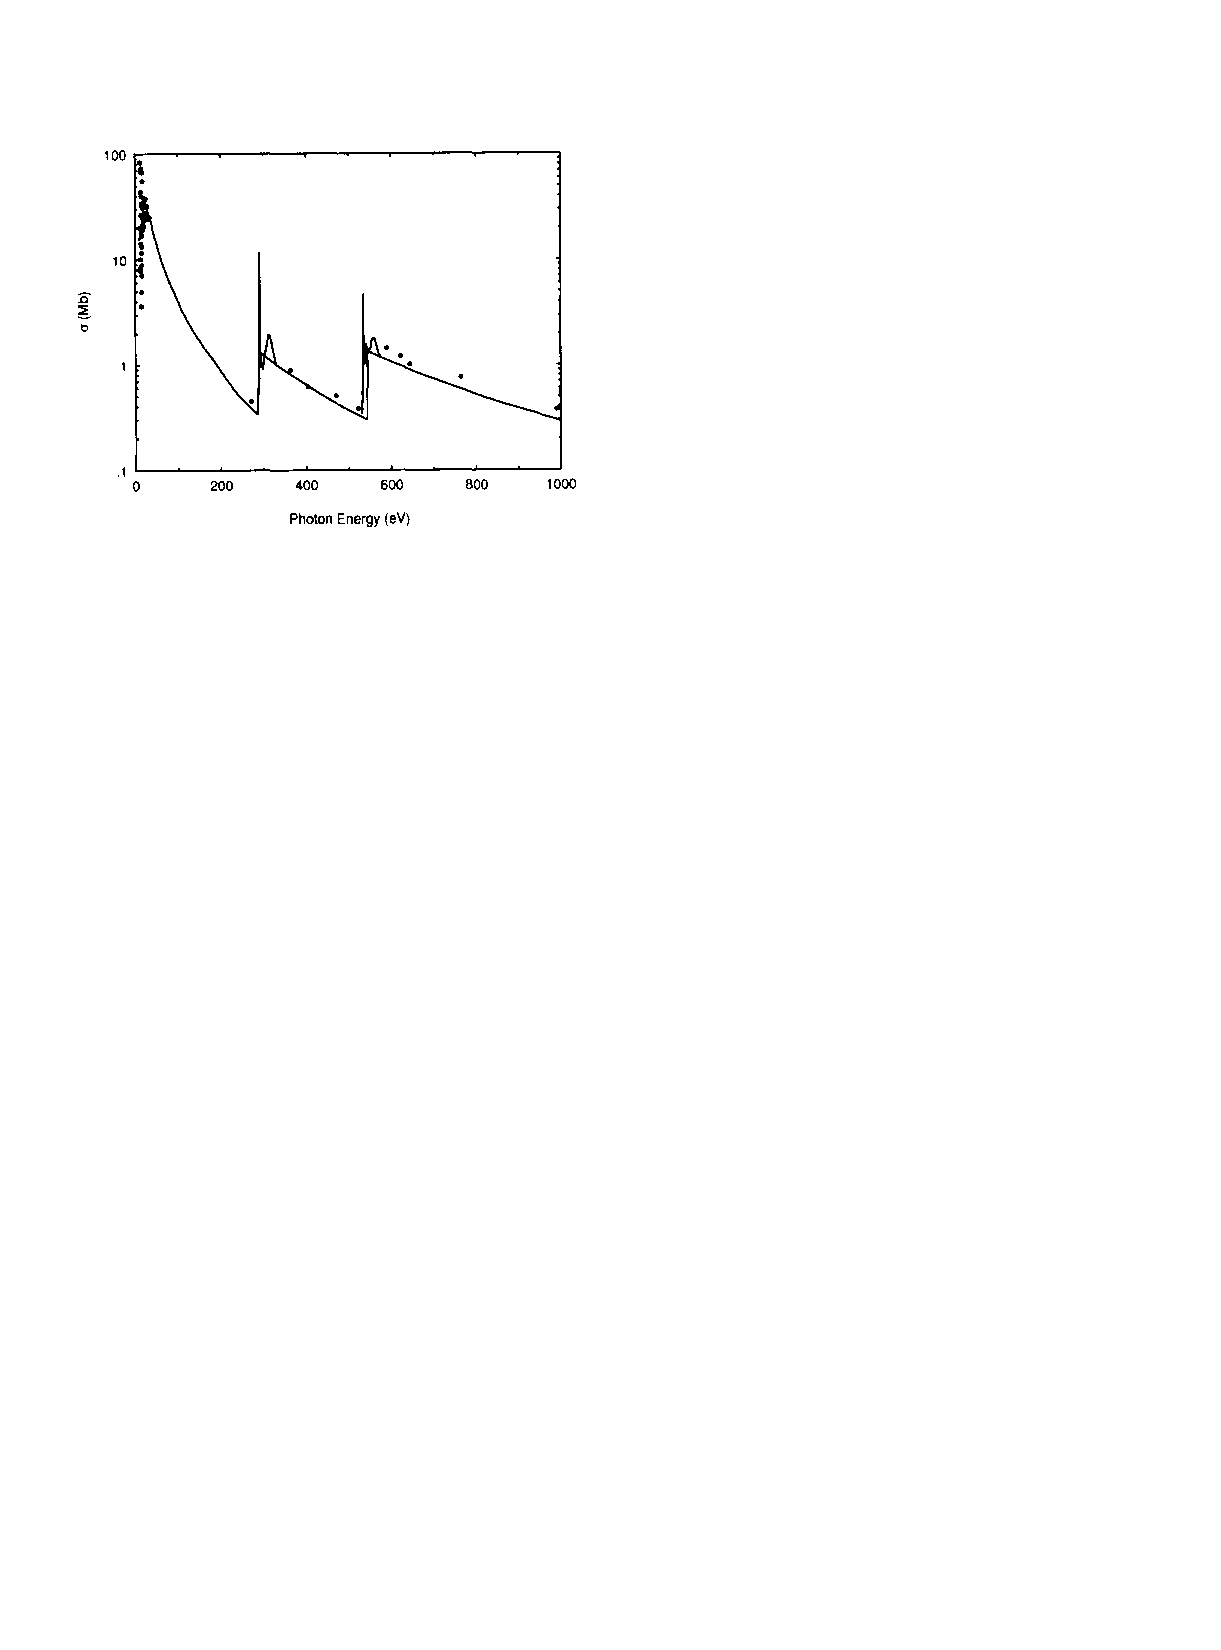
\includegraphics[width=4in]{Chapter2/2f_henke/CO2.pdf} 
   \caption[Experimental photoabsorption data for the CO$_2$ molecule, compared with a plot calculated using the vector sum of atomic photoabsorption cross sections from the Henke tables.]{Experimental photoabsorption data for the CO$_2$ molecule, compared with a plot calculated using the vector sum of atomic photoabsorption cross sections from the Henke tables. The near-edge fine structure causes differences in the vicinity of the C K 1s (284 eV) and O K 1s (543 eV) absorption edges.  Reprinted from Reference \protect \cite[Figure 15]{Hen93}.}
   \label{henkeValid2}
\end{figure}

Far away from absorption edges, the semi-empirical nature of the data gives us a high degree of trust in the accuracy of the Henke-based refractive indexes; however, we need to remember that they do not reflect reality in the vicinity of a material's absorption edges.

The Center for X-ray Optics website \cite{CXR11} offers an online calculator to calculate the refractive index of a compound material using Equation \eq{nFromScatteringFactor} based on its chemical formula and density, subject to the atomic-like assumption.  We used this service to build a database of complex refractive indexes for common grating materials over the 50 eV to 10,000 eV range.  These values were used in all calculations shown later in the text.  In Section TODO, we examine the effect that potential errors in the refractive index would have on the efficiency results.
